\documentclass[12pt]{article}
\usepackage[pdftex]{graphicx}
\usepackage{multicol}
\usepackage{html,makeidx}
\usepackage{amsmath, amsthm}
\usepackage{amssymb}
\usepackage[subfigure]{ccaption}
\newtheorem{theorem}{Theorem}[section]
\newtheorem{lemma}[theorem]{Lemma}
\newtheorem{proposition}[theorem]{Proposition}
\newtheorem{corollary}[theorem]{Corollary}
\newtheorem{definition}[theorem]{Definition}
\newtheorem{conjecture}[theorem]{Conjecture}
\parindent 0in
\parskip 0.1in
\title{Delaunay triangulations and combinatorial Ricci flows}
\pagestyle{plain}
\author{Alex Henniges \\ Thomas Williams \\ Mitch Wilson \\ \\ University of Arizona Undergraduate Research Program\\
Supervisor: Dr. David Glickenstein\\
}

\begin{document}

\maketitle
\hangcaption{}
\thispagestyle{empty}
\newpage
\renewcommand\contentsname{Table of Contents}
\tableofcontents

\newpage
\section{Introduction}

The purpose of this project is to learn about recent developments in discrete differential geometry and produce results, new conjectures, and visualizations. We did this by implementing known and new algorithms and flows computationally. Our program is written in C++. 

We begin in \S\ref{Triangulationschap} with an introduction to triangulations and an explanation of how our program is structured. We then present our research on particular types of triangulations, known as Delaunay triangulations, in \S\ref{DT}. Section \ref{RBk} follows with an explanation of combinatorial Ricci flow along with results from our experiments. In \S\ref{HypSphere} we continue the exploration of combinatorial Ricci flow under different geometries. Lastly, in section \ref{Future}, we provide areas of future research relating and expanding the two subjects.

\section{Triangulations}
\label{Triangulationschap}

\subsection{Basics and Definitions}
\label{BaD}

\begin{definition}
\label{tridef}
A triangulation in \textit{n} dimensions, written $\tau = \{\tau_0, \tau_1, ... , \tau_n\}$, consists of lists of simplices $\sigma^k$, where the super-script denotes the dimension of the simplex and $\tau_k$ is the list of all \textit{k}-dimensional simplices $\sigma^k = \{i_0, ... , i_k\}$. We shall refer to 0-dimensional simplices as vertices, 1-dimensional simplices as edges, and 2-dimensional simplices as triangles or faces \cite{Dave}.
\end{definition}

In this paper, it will not be necessary to work outside of two dimensions. For that reason, we will refer to the spaces being triangulated simply as surfaces.

In two dimensions, we think of a triangulation as a surface that is made up of triangles joined along edges. Traditionally, triangulations are not allowed to have two $k$-simplices sharing the same $k$ vertices. We use a more generalized definition that allows this. Because of this, to define our surfaces we must provide a description for each simplex. In addition to the list of all simplices, for every $\sigma^k$, we must include a list of simplices local to $\sigma^k$. When it is not ambiguous, we will refer to a simplex simply as a set of vertices which it contains.
 
 We define locality as follows:
 \begin{enumerate}
 \item Locality is symmetric. That is, if one simplex is local to another simplex, then that simplex is also local to the first simplex.
 \item If $\sigma^k\subset\sigma^l$, then $\sigma^k$ is local to $\sigma^l$.
 \item If $\sigma^k_1\subset\sigma^{k+1}$ and $\sigma^k_2\subset\sigma^{k+1}$, then $\sigma^k_1$ is local to $\sigma^k_2$.
 \item If $\sigma^k_1\cap\sigma^k_2 = \sigma^{k-1}$, then $\sigma^k_1$ is local to $\sigma^k_2$.
 \end{enumerate}

The number of edges local to a given vertex is also known as the \textit{degree} of that vertex.

In two dimensions, 
\begin{itemize}
\item An edge $\{i, j\}$ is local to vertices \textit{i} and \textit{j}. A face $\{i, j, k\}$ is local to vertices \textit{i}, \textit{j}, and \textit{k}, and edges $\{i, j\}$, $\{i, k\}$, and $\{j, k\}$.
\item Similarly, a vertex \textit{i} is local to all edges that meet at \textit{i} and all faces that meet at \textit{i}. An edge $\{i, j\}$ is local to all faces that meet at $\{i, j\}$.
\item A vertex \textit{i} is local to all vertices that share an edge with \textit{i}.
\item An edge $\{i, j\}$ is local to all edges local to vertices \textit{i} and \textit{j}.
\item A face $\{i, j, k\}$ is local to all faces that share edges $\{i, j\}$, $\{i, k\}$, and $\{j, k\}$.
\end{itemize}

In addition to lists of local simplices, each simplex has information needed to form a geometric triangulation. Namely, each edge $\{i, j\}$ is given a length $l_{ij}$ and each vertex $i$ is given what we call a \textit{weight}, denoted by $r_i$. We think of the weight of a given vertex to be the radius of a circle centered at that vertex. For any $k$-dimensional simplex, there exists an $(k-1)$-dimensional sphere that is orthogonal to each of the spheres centered at the vertices which define that particular simplex \cite{Dave}. The center of this sphere will be called the center of the simplex, denoted by $C(\sigma^k)$.

 For an edge $\{i, j\}$, we define \textit{local length} $d_{ij}$ at vertex $i$ as the distance from vertex $i$ to $C(\{i, j\})$. It is clear that
$$l_{ij} = d_{ij} + d_{ji}.$$
 It can be shown that
\begin{equation}
d_{ij} = \frac{l_{ij}^2 + r_i^2 - r_j^2}{2l_{ij}}
\label{eq2}
\end{equation}
and
\begin{equation}
\label{eq1}
d_{ij}^2 + d_{jk}^2 + d_{ki}^2 = d_{ji}^2 + d_{kj}^2 + d_{ik}^2
\end{equation}

 for any face $\{i, j, k\}$. This proves that for every face $\{i, j, k\}$, the perpendiculars from each edge center meet at a single point, which is the center of the face $C(\{i, j, k\})$ as defined above \cite{Dave}.

There are two notable examples of choices of weights and their corresponding face centers. The first is when all of the weights are zero. In this case, the triangle center $C(\{i, j, k\})$ is the center of the circumcircle of $\{i, j, k\}$. The second is when the weights are equal to the local lengths for \textit{i}, or for all vertices \textit{j} and \textit{k} that are local to \textit{i}, we have $d_{ij} = d_{ik}$. This case is known as a \textit{circle packing} and will be used in $\S\ref{RBk}$. In this case, the triangle center $C(\{i, j, k\})$ is the center of the incircle of $\{i, j, k\}$.

We will now make definitions for the \textit{duals} of our simplices. First, the dual of a face is simply its center $C(\{i, j, k\})$ as defined above. Now we will define a dual for a given edge. Let us refer to any edge, along with its local faces, as a \textit{hinge}. We are able to embed any hinge in the plane. Because of (\ref{eq1}), we know that on any hinge in the plane, the center of an edge along with the centers of its two local faces are collinear. The line connecting these three points is the dual for the given edge. We can determine the length of this dual if we can determine the length of the line segment connecting the center of an edge to the center of one of its local faces. On triangle $\{i, j, k\}$, we write the distance between $C(\{i, j\})$ and $C(\{i, j, k\})$ as 

\begin{equation}
\label{eq3}
h_{ij,k} = \frac{d_{ik} - d_{ij}\cos(\theta_i)}{\sin(\theta_i)}
\end{equation}

 where $\theta_i$ is the angle at \textit{i} on face $\{i, j, k\}$. We refer to this distance as the height of $C(\{i, j, k\})$ with respect to $\{i, j\}$. In the case that $C(\{i, j, k\})$ lies outside of $\{i, j, k\}$ on the side of $\{i, j\}$ where the opposite faces lies, then its height has a negative value. Otherwise, the height is positive \cite{Dave}. Naturally, the dual of a given edge has a distance that is obained by adding the heights of the centers of the faces local to the edge with respect to that edge. The dual of a given vertex \textit{i} is the area enclosed by the duals of every edge local to \textit{i}. The duals of edges will be talked about again in $\S\ref{DT}$.

\subsection{Bistellar moves}

\begin{figure}
\centering
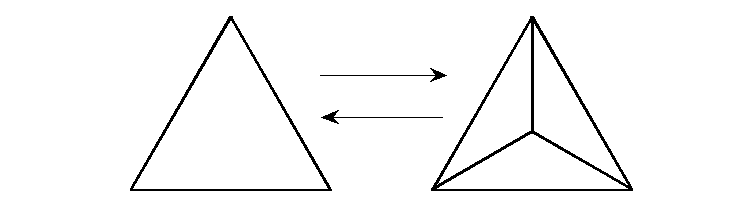
\includegraphics[scale = 0.8]{Pictures3/Flip1331.png}
\caption{The 1-3 and 3-1 moves.}
\label{fig:flip2}
\end{figure}


\begin{figure}
\centering
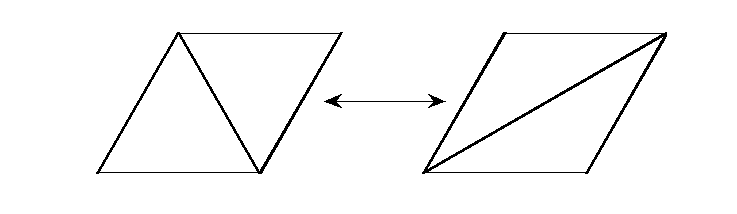
\includegraphics[scale = 0.8]{Pictures3/Flip2.png}
\caption{The 2-2 move.}
\label{fig:flip}
\end{figure}

 On a given triangulation, we are able to perform different modifications, which we will refer to as \textit{bistellar moves} or \textit{flips}. There are three possible bistellar moves that can be performed on a 2-dimensional triangulation: a 1-3 move, a 2-2 move, and a 3-1 move. The 1-3 move and the 3-1 move are inverses of one another while the 2-2 move is its own inverse.

 For the 1-3 move, we consider a face $\{i, j, k\}$. We create a new vertex \textit{l} and place it inside of $\{i, j, k\}$. From this, we create edges $\{i, l\}$, $\{j, l\}$, and $\{k, l\}$. By doing this, we have turned $\{i, j, k\}$ into three new faces, $\{i, j, l\}$, $\{i, k, l\}$, and $\{j, k, l\}$ (see fig. \ref{fig:flip2}). The 3-1 move is simply the inverse of this move. We start by taking a vertex \textit{l} of degree 3 and removing it from the triangulation, essentially removing three faces and three edges with it and leaving behind a single face $\{i, j, k\}$. A 2-2 move is one that requires no additions or removals of any simplices. Consider a hinge with edge $\{i, j\}$ and faces $\{i, j, k\}$ and $\{i, j, l\}$. In a 2-2 flip, we simply take edge $\{i, j\}$ and replace it with a new edge $\{k, l\}$ (see Fig. \ref{fig:flip}). This move will be used extensively in $\S\ref{DT}$.

\subsection{Programming Structure}

 When creating the program, the data structure design was critical. The design not only helps dictate the direction of the project over the course of its lifespan, but the decisions affect the speed and efficiency of all added functionality. Some of the highest priorities of our program are:
 
\begin{itemize}
\item Fast calculations.
\item Easy access to data.
\item Adaptable to a number of situations.
\end{itemize}

\begin{figure}
\begin{center}
\includegraphics[scale = 0.47]{Pictures3/triangulationUML.png}
\end{center}
\caption{A UML diagram of the program. The UML shows how the various files interact as well as the functions and variables they hold. We will refer to many of these programs later on.}
\label{triUML}
\end{figure}

 As seen in Figure~\ref{triUML}, all simplices are assumed to have lists of references to their local simplices broken down by dimension. Each simplex has lists of local vertices, local edges, and local faces. The lists are vectors of integers. The vector, provided in the C++ library, was chosen so that the list can dynamically change in size. The integers are a decision based on both speed and size. Instead of, for example, a vertex having a list of actual edges ($\overline{AB}, \overline{CF},$ etc.) or pointers to edges, the vertex has a list of integers representing the edges. The actual edges are then obtained through the $Triangulation$ class, which holds maps from integers to simplices. The $Triangulation$ class consists of static functions and maps and is designed so only one triangulation exists at any time. Because the maps are static, they can be accessed from anywhere in the code without the need to pass pointers through function calls. Maps also have quick access time.

 In order to build the triangulations that we need for our tests, we decided upon a format that could be entered into a file and then read by our program. This format can be seen in Table~\ref{tab:format}. While this format works fine and we can create some basic triangulations by hand, it is not easy for creating a wide array of triangulations.

\begin{table}
\begin{center}
\begin{tabular}{|l|l|l|}
\hline
 Vertex: 1 &    Edge: 1 &    Face: 1 \\ \hline 

     2 3 4 &        1 2 &     1 2 3  \\

    1 2 4  & 2 3 4 5 7  &     1 2 3  \\

    1 2 3  &       1 2  &     2 3 4  \\ \hline 

 Vertex: 2 &    Edge: 2 &    Face: 2 \\ \hline

   1 3 4 5 &        1 3 &     1 2 4  \\

  1 3 5 7  & 1 3 4 6 8  &     1 4 5  \\

  1 2 4 5  &       1 3  &     1 3 5  \\ \hline 

 			\vdots & \vdots & \vdots \\ \hline 

 Vertex: 5 &    Edge: 9 &    Face: 6 \\ \hline

     2 3 4 &        4 5 &     3 4 5  \\

    7 8 9  & 4 5 6 7 8  &     6 8 9  \\

     4 5 6 &       5 6  &     3 4 5  \\
\hline
\end{tabular}
\end{center}
\caption{The format used to represent a triangulation in our program.}
\label{tab:format}
\end{table}

 Frank Lutz, creator of The Manifold Page \cite{lutzmanifold}, has a catalog of almost two million manifold triangulations of varying sizes. However, the format is different than our setup, so we developed an algorithm to take a given triangulation, saved on its own as a text file, and convert it into the form that we use. We were able to transform this
  
\begin{verbatim}{manifold_lex_d2_n5_o1_g0_#1=[[1,2,3],[1,2,4],[1,3,4],
[2,3,5],[2,4,5],[3,4,5]]},
\end{verbatim}
 
which solely documents the faces, into our format. The result is shown in Table~\ref{tab:format}. 

 These functionalities of our code form the cornerstone for the rest of the program and have to be the most adaptable to future needs, both seen and unseen. Information on other important aspects, like calculating angles, displaying triangulations, and useful objects like points and lines can again be found in Figure~\ref{triUML} or in later sections. 

\section{Delaunay triangulations}
\label{DT}

\subsection{Definitions}
\label{DTD}

 One special type of triangulation is known as a \textit{Delaunay triangulation}, of which there are two different types. The first type is the case of non-weighted triangulations, which we simply call ``Delaunay'', while the second type is reserved for weighted triangulations, which we refer to as ``weighted Delaunay''. We will refer to the condition of not being Delaunay as non-Delaunay and the condition of not being weighted Delaunay as non-weighted-Delaunay. Before we can define what it means for a triangulation to be Delaunay or weighted Delaunay in a global sense, we must define what it means for a triangulation to have either of these conditions in a local sense, and in order to do that, we must consider a single hinge.

\begin{figure}
\centering
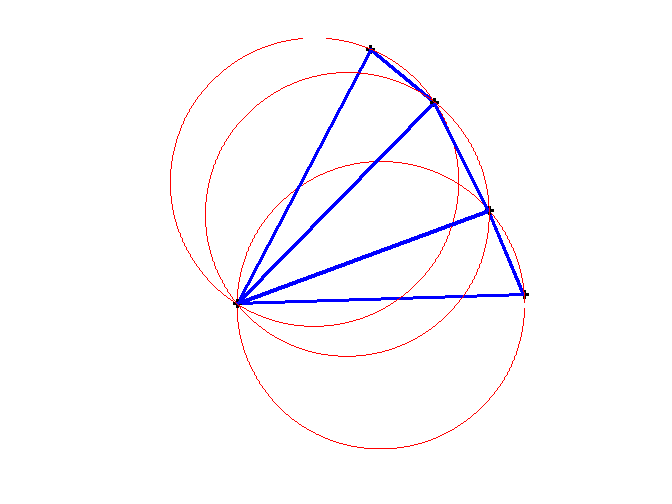
\includegraphics[scale = 0.6]{Pictures3/genTri4.png}
\caption{A simple example of a Delaunay triangulation. The circumcircles are drawn along with the edges to show their compatibility. This is a non-weighted case.}
\label{genTri}
\end{figure}


\begin{definition} A hinge is said to be Delaunay if it cannot fit entirely inside the circumcircle of either of its faces.
\end{definition}

To determine if a hinge is Delaunay, we must consider the circumcircles of both of the triangles in the hinge. In the non-weighted case, this is the circumcircle of the triangle. If the circumcircle of either of these triangles (and as it turns out, necessarily both of them) contains the opposite vertex in the hinge, then we say that the hinge is not Delaunay. However, if both triangles have circumcircles that do not contain the opposite vertex on the hinge, then the hinge is Delaunay. Note that all non-convex hinges, that is all hinges with one of the angles on the edge having a measure greater than $\pi$, are Delaunay.
 
\begin{proposition}
\label{NonDelProp}
The sum of the opposite angles on a non-Delaunay hinge is greater than $\pi$.
\end{proposition}

\begin{corollary}
\label{FlipProp}
Any non-Delaunay hinge will become Delaunay after a 2-2 flip is performed on it.
\end{corollary}

 This proof is given in \ref{prop1}. Note that in the ``boundary case'', the hinge forms a cyclic quadrilateral, i.e. all the vertices lie on the same circle. This occurs when the centers of the triangles, given by the centers of their orthocircles, lie on the same point. In such a case, both the original and the flipped hinge are considered Delaunay.

 The condition of a hinge being weighted Delaunay is somewhat different. As stated before, the dual of a hinge is found by connecting the centers of the two orthocircles. Its length can be found by adding up the two heights. Thus, for two faces, $\{i,j,k\}$ and $\{i,j,l\}$, the length of the dual on the hinge is given by

$$\star\{i,j\} = h_{ij,k} + h_{ij,l}$$

 Recall that a height is measured as negative if the center of the triangle lies on the opposite side of the hinge. Since one or both heights may be negative, we obtain the following:
\begin{definition}
In the case of a weighted triangulation, a hinge is weighted Delaunay when the dual has positive length. If the dual has negative length, then it is non-weighted-Delauany. 
\end{definition}

 A hinge that is nonconvex can also be not weighted Delaunay. This creates issues when one wishes to perform flips on hinges that are non-weighted-Delaunay. It is not entirely clear how one goes about performing a flip on a hinge that is nonconvex. Figure \ref{AntiTri} shows such a hinge before the flip is performed next to the resulting image of a triangle with an ``anti-triangle'' lying over a portion of it. We consider this triangle to have negative area, its angles to have negative measure, and its heights, when otherwise considered positive, to be of negative length.

\begin{figure}
\label{antitri}
\centering
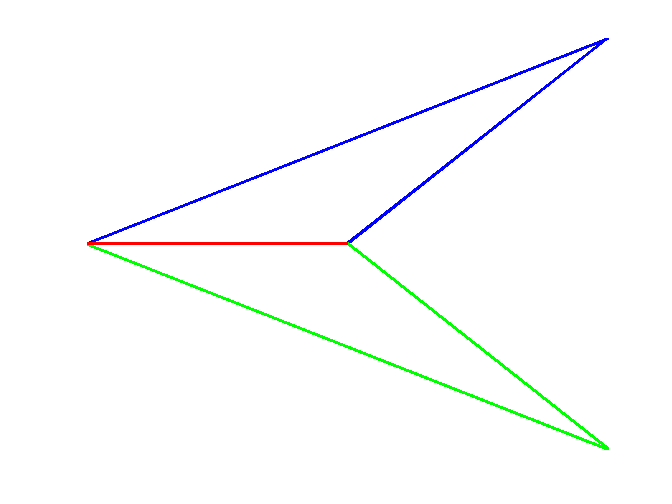
\includegraphics[scale = 0.4]{Pictures3/antitri1.png}
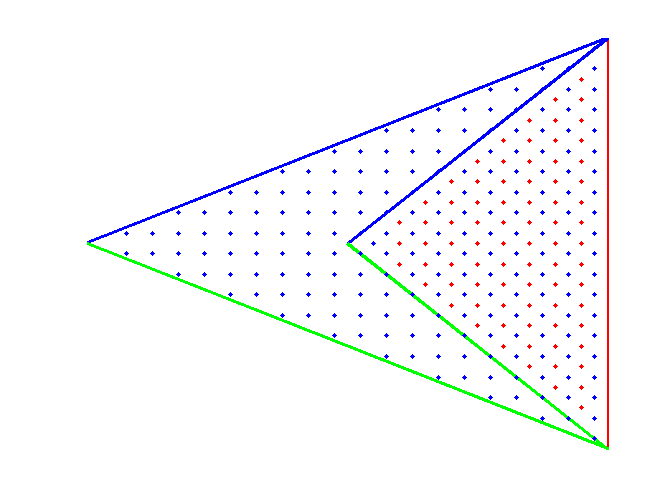
\includegraphics[scale = 0.4]{Pictures3/antitri2.png}
\caption{If flips are performed on a nonconvex hinge, we create an anti-triangle, shaded here in red, and a larger regular triangle, shaded in blue.}
\label{AntiTri}
\end{figure}

 There are a number of remarks to be made regarding negative triangles in our triangulations. First of all, we can give all of our triangles a score, based on their positive or negative orientation, of either 1 or -1. Using this, we can create a value for any point covered by the boundary of a given triangulation. Regardless of the number of flips performed, where, or how many negative triangles are created from them, if one were to pick any point within the pre-existing boundary, the value is guaranteed to be 1. That is to say, for every negative triangle or set of negative triangles created, there is a positive or set of positive triangles created to completely cover them. Additionally, if there is a nonconvex hinge that lies on the border that is flipped where the newly created edge lies outside of the original boundary, the value for every point in the area between this edge and the original boundary will remain 0. From this, we can conclude that the area of any triangulation is preserved under 2-2 flips.

\begin{proposition}
\label{weidelprop}
Any hinge that is non-weighted-Delaunay will become weighted Delaunay after a 2-2 flip is performed on it.
\end{proposition}

 A proof for this is given in $\S\ref{prop2}$. From this we have developed a conjecture.

\begin{conjecture}
\label{flipConj}
Given an arbitrary triangulation in the plane with randomly assigned weights, one can create a weighted Delaunay triangulation through a series of 2-2 flips.
\end{conjecture}

 The goal from this point forward for this part of the project is to write a computer algorithm that effectively asserts this conjecture.

\subsection{Programming Structure}
 We can produce a non-weighted-Delaunay triangulation using mathematical software like MATLAB. However, less is known about weighted triangulations in general. For this project, we aim to develop an algorithm that can create a valid triangulation, add weights to vertices, and manipulate the faces to produce a weighted Delaunay triangulation.

 An important aspect to properly explore these triangulations is in their generation. We developed a program $generateTriangulation$ which can generate a determined number of faces with a random configuration. To truly test our algorithms and to provide convincing results would require an unbiased way of constructing the triangulations. There are several properties to triangulations that we wish to be randomized, and they include the lengths of each edge, the degree of each vertex, and the weight at each vertex. It is not clear to us if there is a way to provide a truly random generation of triangulations or even if such a system would be desirable, but we feel that the algorithm we chose adequately meets our goals.

 Our random triangulation generator begins with one triangle with edge lengths between $0.0$ and $10.0$. This was chosen arbitrarily as all future weights will be based off of these. Triangles are then created from each edge along the border. When the creation of an edge would result in a vertex's angles summing to greater than $2\pi$, we instead close off the vertex by connecting its two outer edges. Once the desired number of faces have been created, the algorithm ends. Figure~\ref{genTris} shows two results of this algorithm.

\begin{figure}
\centering
\includegraphics[scale = 0.45]{Pictures3/gentri.png}
\includegraphics[scale = 0.45]{Pictures3/gentri6.png}
\caption{Two examples of triangulations using our $generateTriangulation$ program, an early version (left) and a modern version (right). Our newer version makes the edge lengths more random, with large and small triangles scattered throughout.}
\label{genTris}
\end{figure}

 We can generate weights at random by restricting their maximum size the weights are not too large. For a given vertex the weight is chosen with respect to the length of the shortest edge local to that vertex. 

 We have created a program called $weightedFlipAlgorithm$ that scans each hinge to check if it is Delaunay, and if not, we perform a flip on it. We repeat the process until each hinge is Delaunay, and thus the whole triangulation is Delaunay. 

 To get a better grasp of the sequence of flips, we made a MATLAB program named $delaunayPlot$ that draws a triangulation so we could visually ensure that our triangulations are being built correctly, see if and where flips were being performed, and track negative triangles. We use MATLAB to generate pictures, including most figures in this paper. We adapted this code to then make $multiDelaunayPlot$, which regraphs the triangulation after a flip is performed. See Figure~\ref{genTri5} for a beginning and end triangulation after going through $weightedFlipAlgorithm$. 

\begin{figure}
\centering
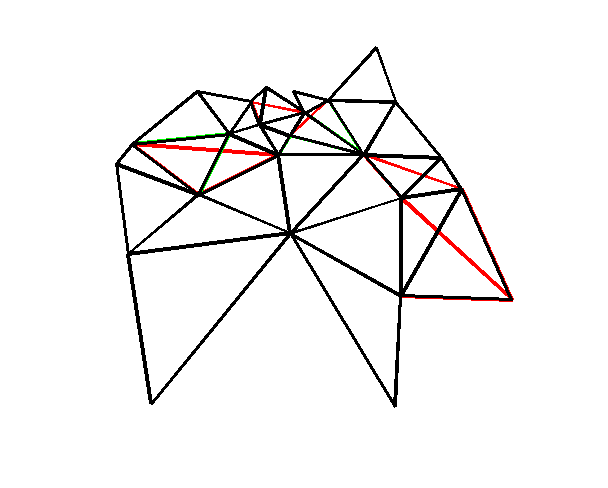
\includegraphics[scale = 0.7]{Pictures3/genTri5v2.png}
\caption{An illustration of our $delaunayPlot$ program. The end triangulation is shown in black. Original edges that were later flipped are shown in red.}
\label{genTri5}
\end{figure}

\subsection{Results}
\label{DTRes}
 Often, we did find that triangulations became Delaunay after a series of flips. As we added more faces and increased the weights, we noted that it was more likely for the algorithm to show flaws. See Table~\ref{DAT}. In watching our $multiDelaunayPlot$ results, we found that certain edges would loop in a series of flips such that performing one flip would require an adjacent edge to need flipping. Occasionally, one edge would get stuck flipping back and forth between two faces. One thing of note was that final triangulations did permit the existence of negative triangles. Often they were found on the edge boundary and of little concern. We were able to check our results by drawing the dual edges on top of all the faces (Refer to our criteria in \S\ref{BaD} and \S\ref{DTD}). If all vertices had zero weight, then the duals are simply the perpendicular bisectors of each edge. See Figure~\ref{Duals}. 


\begin{figure}
\centering
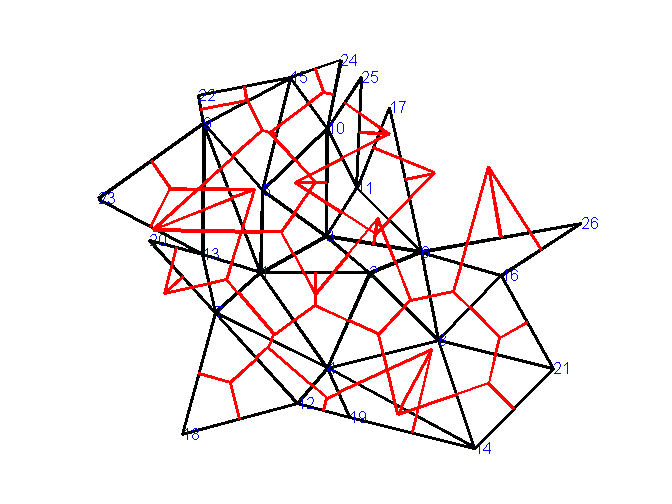
\includegraphics[scale = .45]{Pictures3/nonwduals.png}
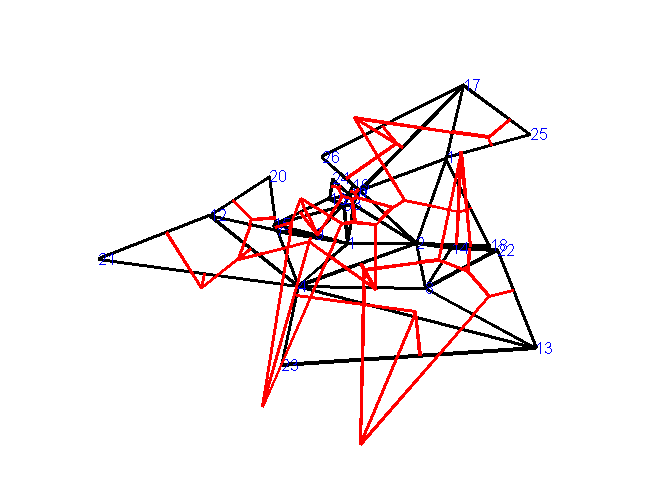
\includegraphics[scale = .45]{Pictures3/Wduals.png}
\caption{A non-weighted (left) and weighted (right) triangulation with dual lengths added.}
\label{Duals}
\end{figure}

 We also observed a couple of interesting things from a experimental point of view. We found that, after flips were performed, the average length of all edges tended to decrease by a small amount. See Figure~\ref{stats} for such an example. There are fewer edges with large weights, and more edges with smaller lengths. This would lead to suggest that vertices try to form triangles with vertices close to itself, resulting in fewer ``skinny triangles''. We also noted that the degrees of vertices sometimes vary more, especially in weighted triangulations; more vertices have a degree of 2 or 3, while others increase in degree. This suggests that the weights of vertices in its triangulation also have a great effect as well as their relative proximities.  
\begin{table}
\begin{center}
\begin{tabular}{|rrr|rrr|}
 \hline
 &Standard weights      &            &            &  Weights increased 50\%           &          \\ \hline

   Faces & Avg. Flips & \% Finish &               Faces & Avg. Flips & \% Finish \\ \hline

        25 &        4.1 &        100 &                    25 &       13.5 &      83.33 \\

        50 &       11.2 &        100 &                     50 &       19.6 &      71.29 \\

       100 &       26.8 &        100 &                   100 &       41.7 &         40 \\ \hline

\end{tabular} 
\end{center}
\caption{An analysis of number of flips required to obtain Delaunay triangulation for a given number of faces and scaled weights. Each test was performed on $weightedFlipAlgorithm$ until each test had ten successful runs. Each trial had unique weights.} 
\label{DAT}
\end{table} 

\begin{figure}
\centering
\includegraphics[scale = 0.6]{Pictures3/Stats.png}
\caption{A statistical illustration of edge lengths and vertex degrees before and after flips are performed.}
\label{stats}
\end{figure}

 In testing our code, we used one particular example to examine a potential special case that may have occurred during the running of our algorithm. The special case, as shown in Figure~\ref{specialCase}, is one where every convex hinge is weighted Delaunay and every nonconvex hinge is not. The results of running our algorithm on this triangulation were of great interest and helped us in further refining the algorithm. When we started, there were seven faces, all positive. When the flip algorithm concluded, we were left with four positive faces and three negative faces. All of the negative faces were paired with positive faces defined by the same three vertices. The remaining odd positive face was defined by the three original boundary edges. This meant that by ``flipping through'' all of the nonconvex hinges, we were left with three pairs of reversely oriented faces, what we also referred to as ``flaps'' or ``double triangles''.

\begin{figure}
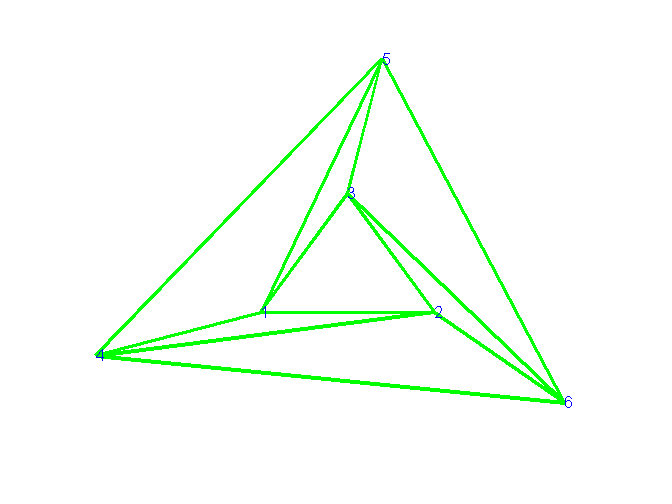
\includegraphics[scale = .45]{Pictures3/triEx1.png}
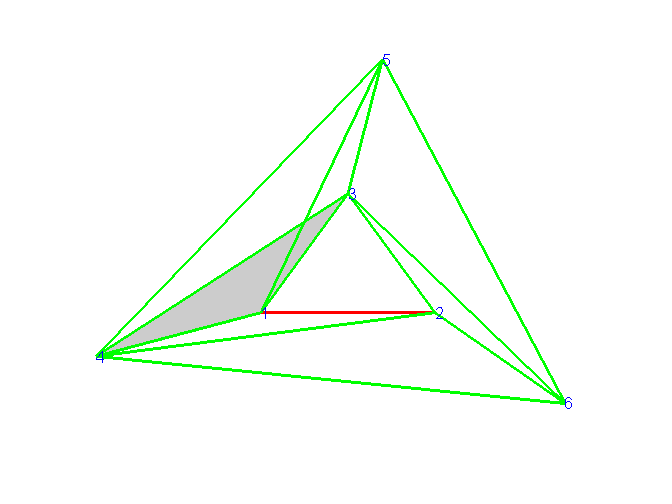
\includegraphics[scale = .45]{Pictures3/triExD1.png}
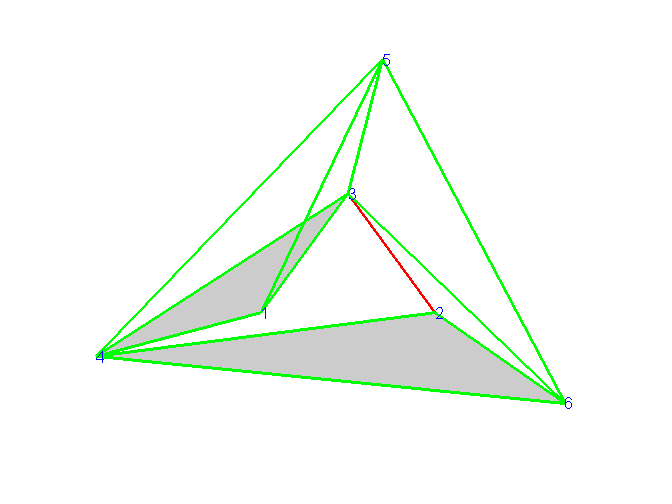
\includegraphics[scale = .45]{Pictures3/triExD2.png}
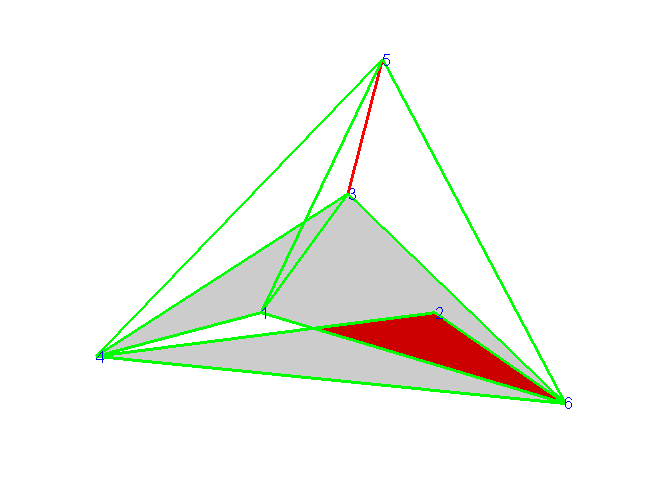
\includegraphics[scale = .45]{Pictures3/triExD3.png}
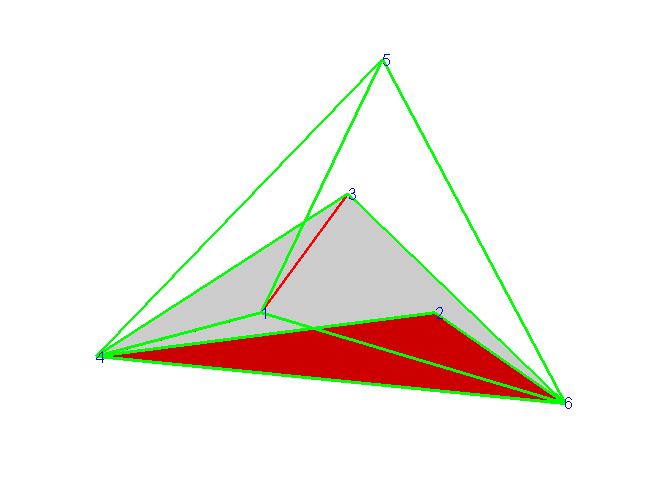
\includegraphics[scale = .45]{Pictures3/triExD4.png}
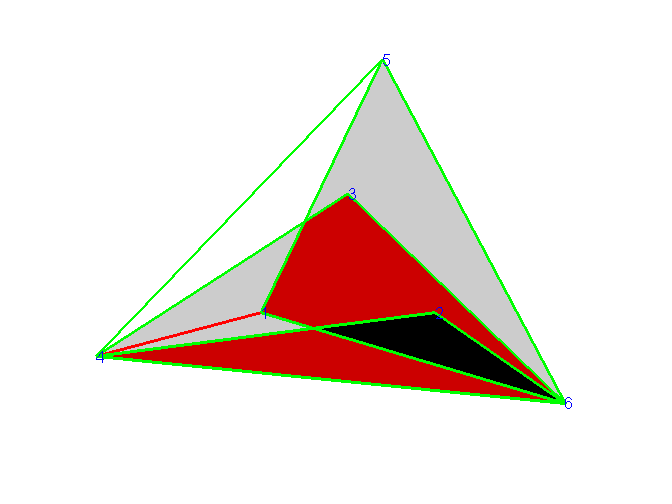
\includegraphics[scale = .45]{Pictures3/triExD5.png}
\caption{Evolution of our special triangulation. Edges that are flipped are shown in red. Negative triangles start off gray, with intersections red. If multiple negative triangles intersect one region, we color it black.}
\label{specialCase}
\end{figure}

The hypothesis was that after any triangulation underwent the transformation of the flip algorithm there would remain only positive triangles or negative triangles that sat opposite of positive triangles lying in the exact same area. The algorithm was modified to simply remove these flaps as a last step to the flip algorithm. This process required removing all vertices that lied at the end of a flap, as well as the edges along these flaps. Finally, the two edges defined by the same two vertices from which these flaps were stemming would be joined into one.

We have not yet run enough tests to make a stronger claim than our conjecture \ref{flipConj}. A significant issue has been the occurence of negative triangles. Without a widely accepted notion of negative triangles, it is still unclear how to handle them in our flip algorithm. Going forward we hope to generalize the cases with negative triangles and address the errors they are causing in our program. But besides such setbacks, we have been able to show that many triangulations with weighted vertices can become Delaunay after a series of flips. 

\section{Combinatorial Ricci flow}
\label{RBk}

Introduced by Richard Hamilton in 1982, Ricci flow, named in honor of Gregorio Ricci-Curbastro \cite{RicciBkgd}, has since had a large influence in the world of geometry and topology. It is often described as a heat equation on geometries. Imagine a room where a fireplace sits in one corner and a window is open on the other side. The heat will diffuse through the room until the temperature is the same everywhere. With Ricci flow, the same occurs with the curvature, which we explain in \S\ref{ricciDef}. Under Ricci flow, a geometric object that is distorted and uneven will morph and change as necessary so that all curvatures are the same. The biggest consequence of Ricci flow came when Grigori Perelman proved the Poincar\'{e} Conjecture in 2002. The Poincar\'{e} Conjecture, proposed in 1904, was particularly difficult to prove, and was one of seven millennium puzzles. Ricci flow turned out to be the cornerstone for the proof. In addition, its relation to the heat equation may open new doors for work in many fields such as fluid dynamics and general relativity \cite{RicciBkgd}. In 2002, Chow and Luo introduced the concept of combinatorial Ricci flow. They showed that this new concept, performed on a triangulation of a manifold, had many of the properties of Hamilton's Ricci flow. The fact that the subject is still very new makes this research project exciting. 

\subsection{Circle-packing}

 Looking back at our weighted Delaunay triangulations, we had the condition that the partial edge lengths were related by Eq.~(\ref{eq1}). As mentioned in \S\ref{BaD}, we will consider circle-packing. Visually, circle-packing entails placing circles with their centers on a vertex so that neighboring circles are tangent to each other. That is, they intersect at only one point, as shown in Figure \ref{rightTri}. Thus, we have the restrictions that $d_{ij} = d_{ik} = r_i, d_{ji} = d_{jk} = r_j,$ and $d_{ki} = d_{kj} = r_k$, ensuring that (\ref{eq1}) holds.

\begin{definition}
A Circle Packing Metric is a distance metric that is an assignment of lengths $l_{ij}$ to all edges $\{i, j\}$ in the triangulation and an assignment of weights $r_i$ (the radius of a circle) for each vertex $i$ such that $r_i + r_j = l_{ij}$. 
\end{definition}

 Choosing to define the geometry in this way, we guarantee the triangle inequality and ensure that we are creating triangles. Note that not all combinations of edge lengths are possible under this system. Some triangulations can simply not be circle-packed. An example is shown in Figure \ref{rightTri}, where there is no combination of weights at the vertices that can make a proper circle-packing. By allowing generalizations of circle-packings, as discussed in $\S\ref{circExt}$, we can broaden our range of possible length assignments.

  
\begin{figure}
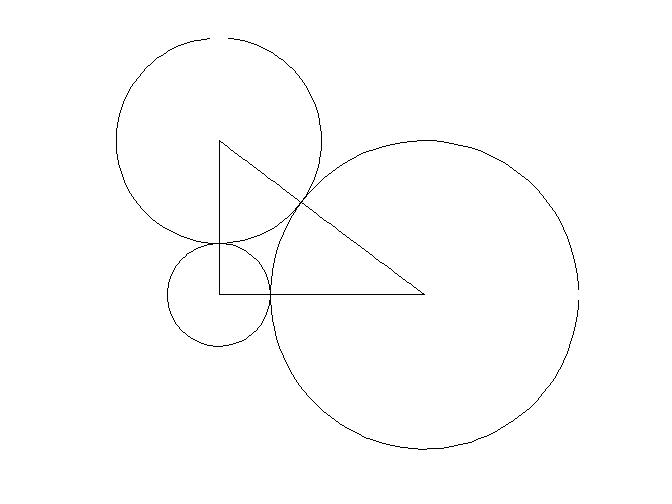
\includegraphics[scale = 0.3]{Pictures3/righttriangulation.jpg}
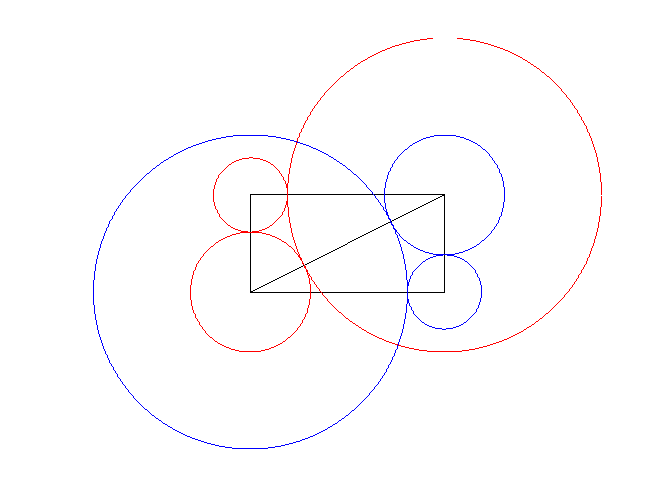
\includegraphics[scale = 0.5]{Pictures3/badcase3.png}
\caption{An example of circle-packing (left) and a triangulation that cannot be circle-packed.}
\label{rightTri}
\end{figure}

\subsection{Definitions and Equations}
\label{ricciDef}

\begin{definition}
A manifold is a collection of points $\mathbb{P}$ such that the neighborhood at every point $p\in\mathbb{P}$ is homeomorphic to the open disk.
\end{definition}

 What this definition means is that around any point of the manifold it appears similar to the sphere. In particular, there are no borders. We refer to this as a closed surface.

 When referring to closed, triangulated surfaces, one important property is the Euler characteristic, $\chi$, defined by $\chi = V - E + F$, where \textit{V} is the number of vertices in the triangulation, \textit{E} is the number of edges, and \textit{F} is the number of faces. This characteristic is directly connected to another important property, the \textit{genus} of a surface. The genus of a surface is the property that is more loosely known as the number of ``holes'' in the surface. For instance, a sphere has a genus of 0 while a torus has a genus of 1, a two-holed torus has genus 2, etc. The relationship between the two values is given by $\chi = 2 - 2g$, where \textit{g} is the genus of the surface. 


\begin{table}
\begin{tabular}{lccccc}
Name  &	Vertices, V &	Edges, E & Faces, F &	Genus, g & $\chi$\\
\hline 
Tetrahedron &	4 &	6 &	4 &	0 & 2\\
Octahedron 	&	6 &	12 &	8 & 0 &	 2\\
Icosahedron &	12 & 30 & 20 & 0	&	 2\\
Torus & 9 & 27 & 18 &	1 & 0\\
Two-holed torus & 10 & 36 & 24 &	2 & -2\\
\end{tabular}
\caption{Listings of vertices, edges, faces, and genus for some common shapes}
\label{EuChar}
\end{table}

 Once we have a triangulation and it is given a Circle Packing Metric, our manifold may not be in a maximally symmetric geometry. We would like to make the geometry uniform. We introduce combinatorial Ricci flow. This equation allows the weights to change over time \cite{chowluo}. The combinatorial Ricci flow is

  \begin{equation}
  \label{Riccif}
  \frac{dr_i}{{dt}} = -K_ir_i
  \end{equation}
  
 where $K_i$ is the \textit{curvature} of a vertex, and $r_i$ is the weight of the vertex $i$. The value of $K_i$ changes with time. We take the sum of all angles associated with a vertex $i$ and define the curvature $K_i$ as

\begin{equation}
K_i = 2\pi - \sum{\angle i}.
\end{equation}

Using side lengths we can determine the angle using the law of cosines. For a triangle with lengths $a, b,\mbox{ and }c,$ the angle opposite side $c$ is
  
  \begin{equation}
  \label{LawOfCosines}
  \angle C = \arccos(\frac{a^2 + b^2 - c^2}{2ab})
  \end{equation}
  
 with similar formulas for the other angles. We see that the system given by (\ref{Riccif}) is highly nonlinear. This equation often results in weights that decrease to zero. Take, for example, a simple tetrahedron with all sides of equal length. We find that the curvature of each vertex always equals $\pi$. Thus in solving the differential equation computationally we would decrease each vertex weight by the same amount, but the curvature of each vertex would still remain $\pi.$ This is because, in the Euclidean case, the curvatures are not affected by uniform scaling. Under (\ref{Riccif}), the radii would continue to decrease until they approach zero length. We have to address this issue since computers don't like working with numbers near zero, as in the denominator of (\ref{LawOfCosines}). Numerical instability may occur. To avoid this issue, we resize the length of each radius by a scalar, $\alpha$. We denote each scaled length by $\tilde{r_i}$ as
 
$$ \tilde{r_i} = \alpha r_i. $$ 
 
 Each $\tilde{r_i}$ would have its own $\tilde{K_i}$, but since we are scaling all sides by the same factor, this does not effect the curvature of the surface, so $\tilde{K_i} = K_i$. Thus in plugging $\tilde{r_i}$ in to the differential equation we get
 
 \begin{eqnarray}
 \label{ref1}
 \frac{d\tilde{r_i}}{dt} &=& \frac{d(\alpha r_i)}{dt} = \alpha \frac{dr_i}{dt} + r_i\frac{d\alpha}{dt}\nonumber\\
 &=& -\alpha K_ir_i + \frac{\tilde{r_i}}{\alpha}\frac{d\alpha}{dt} \nonumber \\
 &=& -\tilde{K_i}\tilde{r_i} + \frac{\tilde{r_i}}{\alpha}\frac{d\alpha}{dt}.
 \end{eqnarray}
 
 We also note that $\displaystyle \frac{1}{\alpha} \frac{d\alpha}{dt} = \frac{d(\log \alpha)}{dt}$ using a basic chain rule. In order to find an appropriate value for $\alpha$ we decided to use the following criterion:
 
\begin{equation}
\label{eqprod}
f(\tilde{r_1},\tilde{r_2},\ldots,\tilde{r_n}) = \prod{\tilde{r_i}} = \prod{\alpha r_i} = C\mbox{, a constant.}
\end{equation}

 We will call this value the \textit{product area} of the surface. This area prevents all radii from decreasing to zero at the same time. By taking the derivative of Eq.~($\ref{eqprod}$) with respect to time we find that 
 
\begin{equation}
\label{proof1}
\frac{d(\mbox{log}~\alpha)}{dt} = \frac{\mbox{sum of all curvatures}}{\mbox{number of vertices}} = \overline{K}, \mbox{average curvature.}
\end{equation}

 In this paper, we may refer to the sum of all curvatures as the \textit{total curvature}. We can also show that $\overline{K}$ is a constant and depends on the number of vertices and the Euler characteristic. We know that the sum of angles on each face is $\pi$, thus we determine that 

$$\sum{K_i} = 2\pi V - \pi F = 2\pi(V - \frac{F}{2})$$

 We can simplify this by noting some basic facts about triangulations of closed surfaces. As every face is made up of three edges, and each edge belongs to two faces, we can see that $3F = 2E, \mbox{or } E = \frac{3F}{2}$. Looking back at Table \ref{EuChar} we note that this is true for all polyhedra listed. Now we rewrite the above equation as

$$\sum{K_i} = 2\pi(V - \frac{F}{2}) = 2\pi(V - \frac{3F}{2} + F) = 2\pi(V - E + F) = 2\pi \chi.$$

 Thus we find that $\overline{K}$ is just $\displaystyle\frac{\sum{K_i}}{|V|} = \frac{2\pi \chi}{|V|}$ where $|V|$ is the number of vertices. This is also noted in \cite{chowluo}. Plugging this information back into Eq.~($\ref{ref1}$) we determine that

\begin{equation}
\frac{d\tilde{r_i}}{dt} = -\tilde{K_i}\tilde{r_i} + \overline{K}\tilde{r_i} = (\overline{K} - \tilde{K_i})\tilde{r_i}
\end{equation}

 However, since everything is now a function of $\tilde{r_i}$ and not $\alpha$, we can just as easily plug $r_i$ back in to the differential equation instead of $\tilde{r_i}$, so we end up with:

\begin{equation}
\label{Riccin}
\frac{dr_i}{dt} = (\overline{K} - K_i)r_i
\end{equation}

 This is known as normalized Ricci flow, as discussed by Chow and Luo \cite{chowluo}. In the case of our basic tetrahedron from earlier, the radii would not change after each iteration as $\overline{K} = K_i = \pi$ and thus $\displaystyle\frac{dr_i}{dt} = 0$ for $i = \{1,2,3,4\}$. 

\subsection{Programming Ricci flow}

 The function $calcFlow$ runs a combinatorial Ricci flow on a triangulation and records the data in a file. The algorithm for solving the ODE, provided by J-P Moreau, employs a Runge-Kutta method of order 4 \cite{JPM}. First, the file name for the data is provided. Then, a $dt$ is given by the user that represents the time step for the system. The next parameter is a pointer to an array of initial weights to use. This is followed by the number of steps to calculate and record. Lastly, a boolean is provided, where $true$ indicates that the normalized differential equation, (\ref{Riccin}), should be used. Otherwise, the standard equation (\ref{Riccif}) is employed. Each step, with every vertex's weight and curvature at that step, is printed to the file. An example is shown in Table~\ref{tab:ricciSteps}.

\begin{table}
\begin{center}
\begin{minipage}{2.2in}
%\begin{multicols}{2}
\begin{tabular}{l|l|l}
\hline
Step 1   & Weight &  Curv\\
Vertex 1:& 6.000 & 0.7442\\
Vertex 2: &3.000 & -1.122\\
Vertex 3:& 3.000 & -1.373\\
Vertex 4:& 8.000 & 1.813\\
Vertex 5: &6.000 & 1.227\\
Vertex 6: &2.000 & -3.046\\
Vertex 7: &4.000 & -0.3045\\
Vertex 8: &8.000 & 1.989\\
Vertex 9: &5.000 & 0.07239\\ \hline
\end{tabular} 
\end{minipage}
\begin{minipage}{2.2in}
\begin{tabular}{l|l|l}
\hline
Step 50 &  Weight &  Curv\\
Vertex 1:& 4.557 & 0.008509\\
Vertex 2: &4.530 & -0.01185\\
Vertex 3: &4.534 & -0.009091\\
Vertex 4:& 4.563 & 0.01268\\
Vertex 5:& 4.550 & 0.002772\\
Vertex 6: &4.527 & -0.01455\\
Vertex 7: &4.541 & -0.003563\\
Vertex 8: &4.559 & 0.01018\\
Vertex 9: &4.553 & 0.004906\\ \hline
\end{tabular}
\end{minipage}
%\end{multicols}
\end{center}
\caption{Two steps of a Ricci flow}
\label{tab:ricciSteps}
\end{table}

 After the initial design of $calcFlow$, tests were run to determine its speed. The time it took to run was directly proportional to the number of steps in the flow. However, it was also proportional to more than the square of the number of vertices of the triangulation. As a result, while a four-vertex triangulation can run a 1000 step flow in three seconds, it would take a twelve-vertex triangulation 43 seconds to run the same flow. After inspecting the speed of the non-adjusted flow in comparison, it became clear that the calculation of total curvature, which should remain constant in two-dimensional Euclidean manifold cases, was being calculated far too often. After being adjusted so that it is calculated just once per step, the speed of the flow is much faster so that a four-vertex system with 1000 steps takes just one second and twelve vertices is much improved with a time of only four seconds. The code for the $calcFlow$ function can be found in $\S\ref{calcFlowCode}$.

\subsection{Initial testing and results}

 Initial checks for correctness:
\begin{enumerate}
\item Boundary of tetrahedron will converge to equal weights.
\item Constant \textit{product area}.
\item Constant total curvature.
\end{enumerate}

We have some expectations for combinatorial Ricci flow on two-dimensional surfaces. Cases like the boundary of the tetrahedron can be calculated by hand so it is useful to test our results against these surfaces. For example, we expect that the tetrahedron under the standard combinatorial Ricci flow (\ref{Riccif}) will have all weights converge to zero. Whereas under equation~(\ref{Riccin}) the weights are expected to converge to positive constants.

 There are other expected behaviors. We expect that the \textit{product area} will be constant at any intermediate step of the flow. Also, it is predicted that the total curvature of a 2-manifold surface should remain a constant determined by its genus.

\subsubsection{First tests}
\label{InitialResults}
The first test was the boundary of the tetrahedron. In the standard equation, it is easily shown that all weights approach zero exponentially fast. We then use the normalized Ricci flow for the rest of the testing. In the normalized equation the tetrahedron's weights approach a single positive number, the fourth root of the \textit{product area} of the tetrahedron, so that the area remains constant. In addition, all the curvatures converged to the same value, in this case $\pi$, so that the total curvature is $4\pi$. Results were similar for the other platonic solids.

 The next test was the torus with a nine-vertex triangulation. Again all the weights approached the same positive number to maintain constant area. As expected, the curvatures all went to zero while the total curvature remained zero throughout. Further simple tests included triangulations of larger genus, and in all cases the total curvature remained at the constant multiple of $\pi$ that was expected and the \textit{product area} was also constant. In addition, there does not appear to be any further effect from the initial weights other than determining the area of the triangulation. It is not clear from any of the tests we ran that having large disparities betweeen the weights (some small while others very large) causes a different end result.

 In each case all vertices converged to the same curvature. This was not always the situation for the weights, as in many triangulations there would be several final weights. It became clear that this would occur when vertices had different degrees. In fact, we guess that there is a formula relating the \textit{product area} of a weighted triangulation and the degree of a vertex to that vertex's final weight. In most of the examples we tried, when two vertices had the same degree, they had the same final weight, but this is not always the case. One such example is adding three vertices to one face of the tetrahedron. As seen in Table \ref{tab:weightTab}, vertices 4, 5, and 6 all have degree four. Yet vertex 5 has a greater final weight than the other two. We believe this is because the local vertices of 5 are different in degree from those of 4 and 6. That is, the degrees of the local vertices of 5 are never less than four, while vertices 4 and 6 each have a local vertex with degree 3. See Figure \ref{fig:t7vh} in the Appendix for an illustration of weights over time. 


\begin{table}

\begin{minipage}[ht]{0.5\linewidth}

\begin{tabular}{|l|l|}
\hline
 Vertex: 1 &  Vertex: 5 \\
\hline
2 3 4 5 6 7  &   1 2 4 6  \\

1 2 3 7 10 13  &  7 8 9 12  \\

1 2 3 5 7 9  &   5 6 7 8  \\
\hline
 Vertex: 2 &  Vertex: 6 \\
\hline
1 3 4 5 6 7  &   1 2 5 7  \\

1 4 5 8 11 14  & 10 11 12 15  \\

1 2 4 6 8 10  &  7 8 9 10  \\
\hline
 Vertex: 3 &  Vertex: 7 \\
\hline
    1 2 4  &     1 2 6  \\

    2 5 6  &  13 14 15  \\

    2 3 4  &    1 9 10  \\
\hline
 Vertex: 4 &  Edge: 1    \\ 
\hline
  1 2 3 5  &   :         \\

  3 4 6 9  &   :         \\

  3 4 5 6  &            \\ 
\hline

\end{tabular}


\end{minipage}
\begin{minipage}[b]{0.5\linewidth}

\begin{tabular}{|l|}
\hline
Final weights for a random \\

initial weighted Triangulation \\
\hline
Vertex 1: 15.692 \\

Vertex 2: 15.692 \\

Vertex 3: 6.18421 \\

Vertex 4: 9.6524 \\

Vertex 5: 10.6409 \\

Vertex 6: 9.6524 \\

Vertex 7: 6.18421 \\
\hline
\end{tabular}
\end{minipage}
\caption{Adding three vertices to a Tetrahedron}
\label{tab:weightTab}
\end{table}


\subsubsection{Morphs and specific cases}

Another part of the code is a file strictly made up of functions used to manipulate and alter the triangulations. These functions, known within the code as \textit{morphs}, allow us to change the triangulation in different ways, geometric as well as topological, in order to provide us with different kinds of discrete manifolds over which to run our flow.

 One such example of our morphs is the use of flips, as mentioned in \S\ref{BaD}. We can perform 1-3, 2-2, and 3-1 flips on given triangulations and observe how those alterations affect the end flow. Flips have the special property that they do not change the Euler characteristic of the surface they are performed upon. For example, in performing a 1-3 flip, we have a total of 3 new edges, 2 more faces, and 1 new vertex. The value of $\chi$ does not change as $(V+1) - (E+3) + (F+2) = V - E + F = \chi$. This means we could do any number of these flips without changing the topology of the surface.

 In addition, there are other ``morphs'' that can be performed to change the topology of a triangulation in order to give us some more diverse and interesting shapes over which to run these flows and observe their results. There are two such moves that we can perform.

\begin{itemize}
\item Adding Handles \newline
By adding a handle to a surface, we are in essence adding a hole to it. One simple way to obtain this result is to ``patch'' the surface of a torus to the surface that we are working with. This is exactly what we have done. The method removes a face from the existing triangulation and replaces it with a 9-vertex triangulation of a torus. By using the three existing vertices and edges, we are actually adding 6 new vertices, 24 new edges, and 16 new faces. This operation changes the topology of the triangulation that we are working with. It will reduce the Euler characteristic, $\chi$, by 2 and thus change the total curvature of the surface.
\item Adding Cross-Caps \newline
The purpose of adding a cross-cap to a manifold is to give us a property of non-orientability. A surface of this kind is characterized by the ability to move an object along it in such a way that it reaches its original location but in mirror-image form. In this way, the portion of the surface known as the cross-cap is, itself, topologically equivalent to the mobius band. It is sufficient to add only a single cross-cap to any given surface. In conjunction with the method of adding handles, this technique allows us to create any topology in two dimensions.
\end{itemize}

We reintroduce here the concept of a \textit{double triangle}, first mentioned in \S\ref{DTRes}. A double triangle is made of two triangles with the same three vertices. As part of a triangulation it can be imagined as flattening a party hat and attaching it to an object along the open end. We wish to observe how they are affected with combinatorial Ricci flow.

% Another shape we have been looking into is called the \textit{double triangle}. A double triangle is made of two triangles with the same three vertices. It can also be thought of as folding one triangle on top of another. We can add these to a triangulation and see how things vary with their presence. This is of interest because of their very peculiar effect on the definition of a triangulation. Without double triangles, there are certain restrictions on definitions and adjacency properties of simplices within a triangulation as outlined in the previous section on triangulations. However, with these double triangles, the restrictions are broken up by allowing double and even triple adjacency references, creating vertices with only one or two local vertices, faces with only two defining edges, and edges with only one defining vertex, among other bizarre properties. Because of these inconsistencies in definition, different surfaces that have these double triangles attached to them will behave in noteworthy ways. The function that adds these shapes takes an edge as an argument and adds another edge with the same two vertices. Then, a vertex is added and two edges are drawn from this vertex to the other two vertices mentioned. Two new faces are formed by these two new edges as well as the other two edges mentioned, one for each face. The process can be imagined as flattening a party hat and attaching it to an object along the open end.

 We investigate our programs for sanctity by performing morphs on given manifolds and observe any changes in behavior. We include some examples. 

 \textit{Example}: Adding a vertex to a one-holed torus. See Figure~\ref{torusaddv}. 

 By inserting a vertex within a triangulation for a torus, we are essentially creating a bump on the torus. We can then observe what happens as we run it through our $calcFlow$ program. The new vertex shrinks in size to a weight much smaller than the other vertices, but to a positive constant. To counter this, the other vertices grow slightly to maintain Eq.~(\ref{eqprod}). In all cases (where the vertices began with different weights), the weight that the new vertex converges to is in a proportion to the other weights by a factor of $3+2\sqrt{3}$, the exact proportion necessary to maintain equal curvature amongst all the weights. An oddity here is that the three vertices local to this added vertex converged to the same weight as all the vertices not near the flip, despite a difference in degree.

\begin{figure}[ht]
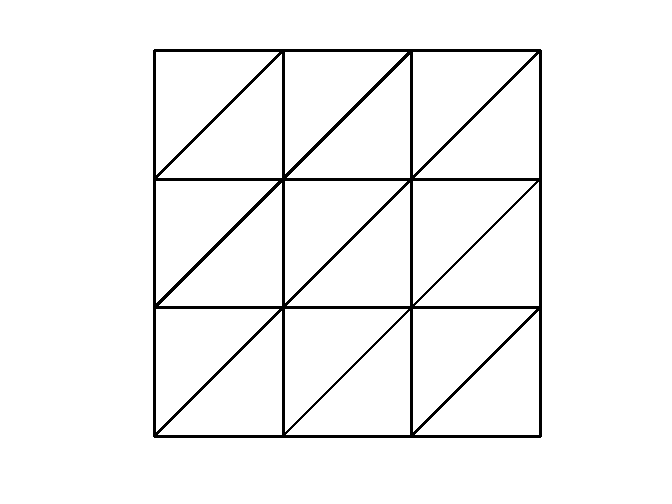
\includegraphics[scale = 0.5]{Pictures3/torus22.png}
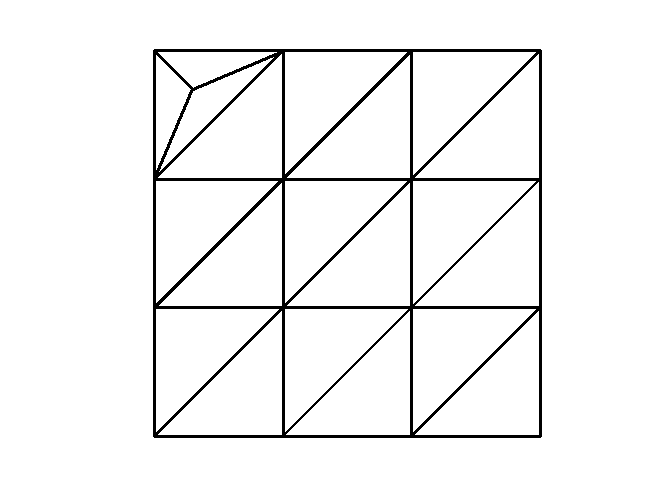
\includegraphics[scale = 0.5]{Pictures3/torus2addvertex2.png}
\caption{A triangulation of the torus, and the addition of a new vertex. This is a 1-3 flip.}
\label{torusaddv}
\end{figure}

 \textit{Example}: Adding a double triangle to a two-holed torus.

When we added a double triangle to the edge of a two-holed torus, we experienced for the first time what is known as a singularity. At the special vertex that was only of degree two, its weight continued to shrink and never converged. Eventually, enough steps of the Ricci flow were performed that the size of the weight became less than what the computer could differentiate from 0 and the program crashed with a division-by-zero error. Before the crash, the other vertices were increasing without convergence to counteract the decreasing weight. The reason is that all vertices wanted to attain the same curvature, in this case $-\frac{2}{5}\pi$. Yet the new vertex, with only two angles in its sum, can only obtain a curvature of 0 (each angle $\sim\pi$ radians). The result is that the weight shrinks in an attempt to attain angles greater than $\pi$, which is simply not possible. What is still not clear is whether or not the weight reaches 0 in finite time, or simply approaches 0. This is difficult to test with a computer only capable of approximating the weight, though we expect that it does so in finite time.

 \textit{Example}: Performing a 2-2 flip on a 12-vertex torus. 

 Flips can drastically change the behavior of some triangulations. For example, in a 12-vertex torus, performing a flip on a particular edge created a double triangle. Similarly to the previous case, all curvatures are converging to 0, but the vertex with degree 2 simply cannot accomplish this. However, unlike the previous case, we suspect that the weight does not become 0 in finite time, but instead approaches 0 in infinite time. See Fig.~\ref{fig:t7vh} for an illustration of how a 1-3 flip and another morph can change the behavior of weights over time.

\begin{figure}[ht]
\centering
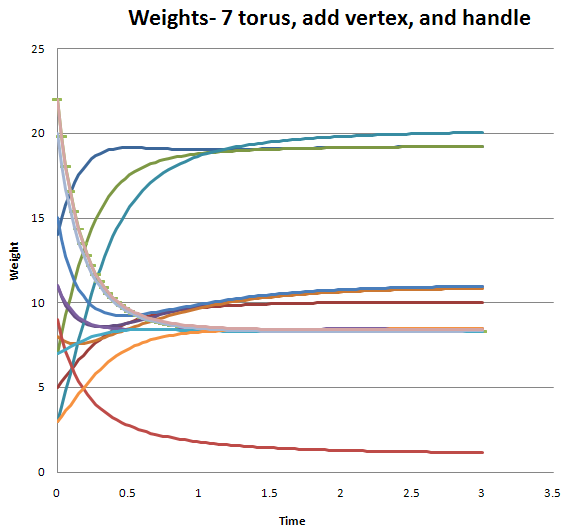
\includegraphics[scale = 0.65]{Pictures3/torus2addvertex2new.png}
\caption{An example of how morphs can change the asymptotic behavior of vertices. In this case we saw the weights of some vertices change concavity.}
\label{fig:t7vh}
\end{figure}

 \textit{Example}: Triangulation of genus 4.

 While the previous two cases were quite interesting, we were using double triangles and being less restrictive in what were allowable triangulations. But in the same sense that a degree two vertex could have a curvature no less than 0, a degree three vertex is bounded below by $-\pi$. It was found that the curvatures of a triangulation are dependent on the number of vertices and the genus, so a triangulation with a large enough genus and few vertices could have its curvatures converge to less than $-\pi$. The first we found, provided by \cite{lutzmanifold}, was an 11 vertex triangulation with genus 4. To create a vertex with degree 3, we chose to add a new vertex to a face with a 1-3 flip. This made all curvatures attempt to converge to $-\pi$. The new vertex reacted as in the previous example, approaching a weight of 0. Whether or not this situation is possible for a vertex of any degree is unknown. To test this one would need a very high genus, but this requires more vertices. Unfortunately, \cite{lutzmanifold} does not provide large enough triangulations to test for vertices with degree greater than three. A similar result can be seen on a genus 6 surface in Figure~\ref{g6}.

\begin{figure}
\centering
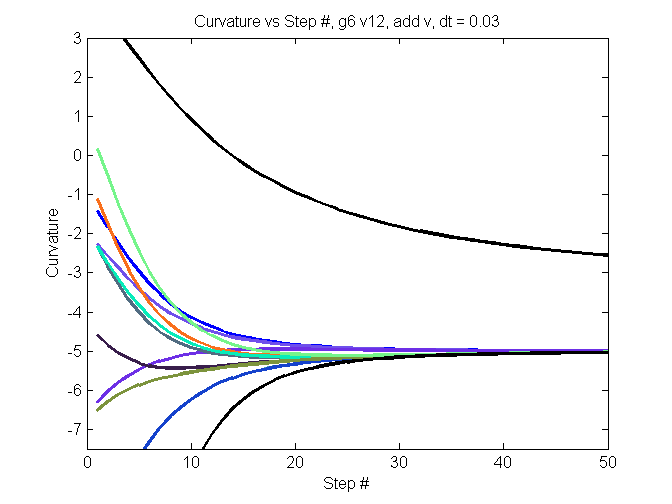
\includegraphics[scale = 0.7]{Pictures3/Curvg6v12addv.png}
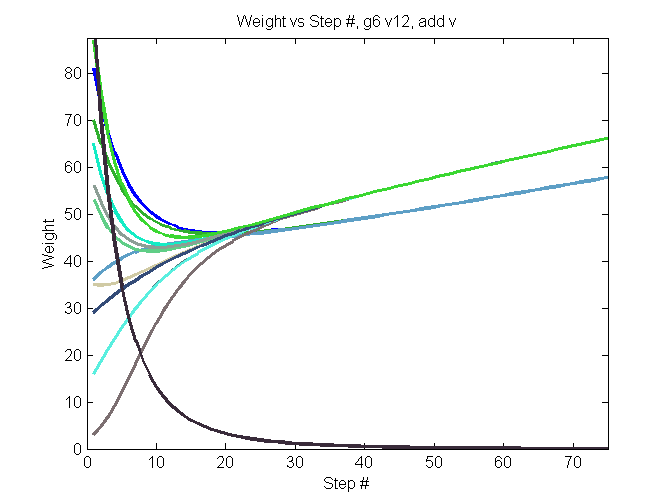
\includegraphics[scale = 0.7]{Pictures3/Weightg6v12addv.png}
\caption{An example of adding a vertex to a genus 6 surface. One of the curvatures in unable to drop below $-\pi$, and as a result, its weight is pushed to almost zero. Other vertices group together to compensate for this behavior.}
\label{g6}
\end{figure}

\textit{Example}: Two tetrahedra connected at a vertex. See Figure \ref{fig:tt}

 It turns out $\chi = $ 7 Vertices - 12 Edges + 8 Faces = 3, which is not a case we had seen before. Technically, this example is not a manifold, but we felt it was useful in validating our program procedure. Starting with equal weights, we obtained a somewhat unexpected result. The center weight becomes very large, and the others become smaller in comparison. We concluded that since the central vertex has a much higher degree, its weight becomes large, creating elongated tetrahedra on either side, in order to have the same curvature as all other vertices.

\begin{figure}
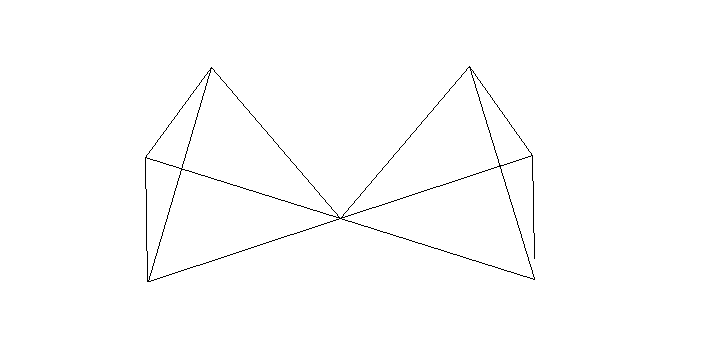
\includegraphics{Pictures3/tetratouch.png}
\caption{Two tetrahedra joined at a vertex.}
\label{fig:tt}
\end{figure}

\subsubsection{Convergence speeds}

One experiment we performed was measuring convergence speeds of various triangulations. For each triangulation, five flows were run where the weights were random between one and twenty-five. Random weights, while not a perfect solution, was the most effective option and easiest to implement. As we do not want weights to be a factor in our convergence speed tests, it was unclear which set weights could have the same effect for different triangulations. By performing five trials and using random weights, we hope to negate any effect the weights could have on the convergence speed of a triangulation. The $dt$ was held constant at 0.03 so that the number of steps needed to run was not large and still provided accurate results. For each run, a step number was assigned for when all weights and curvatures had converged to four digits, (the precision shown in a file of the results).

\begin{figure}
\centering
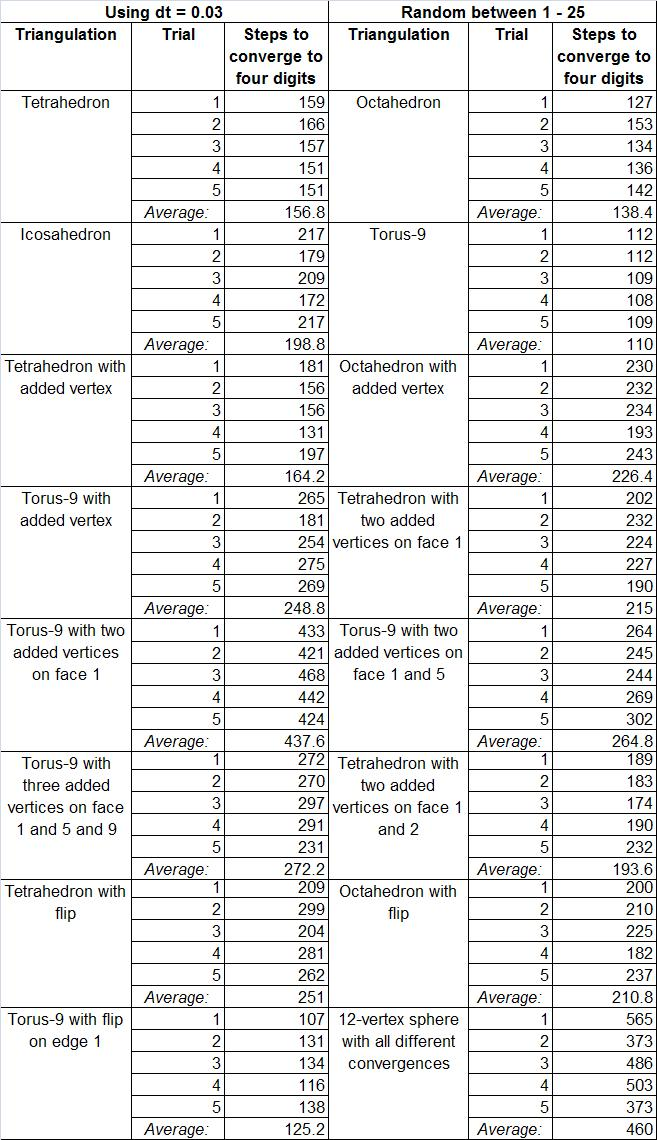
\includegraphics[scale = 0.7]{Pictures3/ConvergenceTable.png}
\caption{Summary of convergence data for varying criteria}
\label{fig:conv}
\end{figure}

 Beginning with the basic case, the tetrahedron took an average of 156.8 steps to converge to four digits and remained fairly consistent through all five trials. Strangely, the octahedron converged faster on all five flows, averaging 138.4 steps. This was made all the stranger by the fact that the icosahedron averaged 198.8 steps. The torus revealed several things about convergences. First, the standard nine vertex torus averaged only 110 steps, suggesting that a torus converges faster than a sphere. When a vertex was added to the torus, it greatly decreased the convergence speed, to 248.8 steps. Compared to the Tetrahedron with an added vertex, 164.2, this was a very large jump. When another vertex was added to the same face as the first, the convergence speed dropped yet again, to an average of 437.6 steps. Yet when this vertex was added to a face not connected to the first, the convergence speed was almost steady at 264.8. And adding a third in the same style caused little increase.

 This seems to suggest that convergence speed is dependent on the number of vertices with the same properties. By the properties of the vertex, we mean the number of local vertices, the weight it converges to, etc. When the vertices were added to separate faces, there remained only three unique sets of properties. Whereas, adding the two vertices to the same face created five unique sets. This theory is further supported by a twelve vertex sphere designed so that all vertices have distinct properties. The average convergence was 460 steps, more than twice as long as the icosahedron, which also is a twelve vertex sphere.

 As a final note, the deviation of the initial weights did not have a clear impact on the convergence speed. At some times, it would appear that initial weights with a higher deviation would converge faster, yet at other times it was lower deviation that seemed to lead to faster convergence.

\section{Spherical and hyperbolic Ricci flow}
\label{HypSphere}

So far we have focused exclusively on triangulations using Euclidean geometry. While this is useful for most cases, there are others where a different background space may be better suited. Two of these in particular are spherical and hyperbolic geometries. We will introduce the basics of each system to readers as they may be unfamiliar with these geometries. We will examine the adaptations of combinatorial Ricci flow for each case, test over various triangulations, and attempt to reach conclusions on our findings. 

\subsection{Spherical flow}
If you were to draw a large triangle on the surface of the earth, you would see that the line segments are no longer linear, but follow along an arc. In dealing with spherical geometry, we learn that many rules of traditional planar geometry, some of them fundamental, do not apply. To begin, the sums of angles in a triangle do not add to $180^\circ$. The sum changes depending on the area of the triangle. For computational reasons, we cannot (easily) have edges of unbounded length. While we can assume our circle-packing metric still holds, we do have additional restrictions: 

\begin{itemize}
\item All triangles must be realizable on a sphere of radius 1, the unit sphere. 
\item The sum of the weights of any triangle cannot exceed $\pi.$ As such, no two weights can add up over $\pi$. By circle-packing, each edge length must then be less than $\pi$, therefore we imply the geodesic between any two points, using the shortest distance on the surface between the two vertices. 
\end{itemize}

 We also have different formulas in the spherical case. There are now two laws of cosines. One gives you an angle based on the edge lengths, like in Euclidean space, and the other gives you the side lengths based on the angles. For the first law of cosines, given a triangle with edge lengths $a, b$, and $c$, we have $\cos(\angle C) = \frac{\cos(c) - \cos(a)\cos(b)}{\sin(a)\sin(b)}$. Using Taylor polynomials to a couple of terms, we can see that the spherical law of cosines approaches the Euclidean version in its limit. With $\sin(x) \approx x$ and $\cos(x) \approx 1 - \frac{x^2}{2}$ for $x$ small, we get 
\begin{eqnarray*}
\cos(\angle C) &=& \frac{\cos(c) - \cos(a)\cos(b)}{\sin(a)\sin(b)} \approx \frac{(1 - \frac{c^2}{2}) - (1 - \frac{a^2}{2})(1 - \frac{b^2}{2})}{ab}\\
							&=& \frac{\frac{a^2}{2} + \frac{b^2}{2} - \frac{c^2}{2} + \frac{a^2b^2}{4}}{ab}\\
							&=& \frac{a^2 + b^2 - c^2}{2ab} + \frac{ab}{4} \approx \frac{a^2 + b^2 - c^2}{2ab}.
\end{eqnarray*}

 More importantly, our equation for combinatorial Ricci flow is altered slightly. The base equation, as given by \cite{chowluo}, is now 
\begin{equation}
\label{SRiccif}
\frac{dr_i}{dt} = -K_i\sin(r_i).
\end{equation}

\begin{figure}
\centering
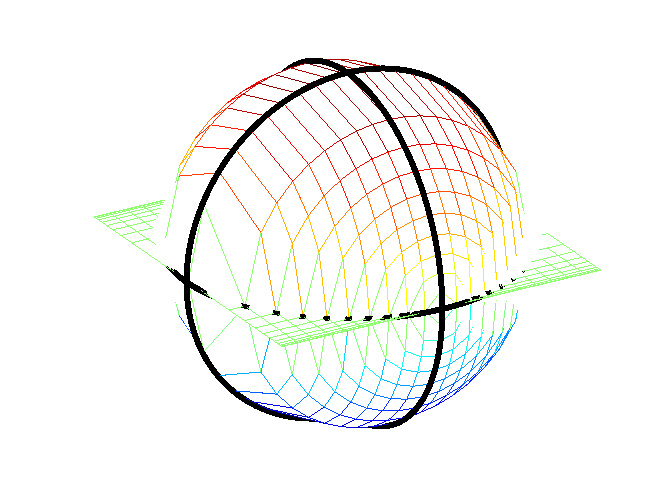
\includegraphics[scale = 0.6]{Pictures3/octosph.png}
\label{OctoSph}
\caption{An illustration of a spherical octahedron through the X-Y plane. Each octet of the sphere surface, outlined in black, is the face of one triangle.} 
\end{figure}

 Like in the Euclidean case, we see the possibility that all weights could continually decrease towards zero. However, scaling in the spherical case is not quite as easy as before: the angles are affected by the change in edge lengths. We also need to make sure that the weights remain within bounds.

 We tried a few techniques to derive an equation for normalized spherical flow. Some ideas were:

\begin{itemize}
\item $\displaystyle \frac{dr_i}{dt} = (\overline{K} - K_i)\sin(r_i)$ \newline
 By maintaining the same construction as the normalized Euclidean Ricci flow, we hoped that replacing $r_i$ with $\sin(r_i)$ would work. However, in running even the simplest case of a tetrahedron, we found that the system was highly unstable. If more than one weight was initially different from the others, the program would fail. If the system was able to stabilize, we noted that the resultant surface area of the end product was $4\pi$, the same as a unit sphere. Another issue with this formula is that the value $\overline{K}$ is no longer constant. For a spherical construction of a surface $X$, we have 

$$\overline{K} = \frac{\sum{K_i}}{|V|} = \frac{2\pi\chi - \mbox{Surface Area of }X}{|V|}.$$

 This is known as the Gauss-Bonnet theorem and is noted by Chow and Luo \cite{chowluo}. Since the surface area went to $4\pi$, then the average curvature went to zero. 

\item $\displaystyle \frac{dr_i}{dt} = (\hat{K} - K_i)r_i$ \newline
 Following the criteria we used to obtain our normalized Euclidean flow, we began experimenting and used the cases $\tilde{r_i} = \alpha r_i$ and $\prod{\alpha \sin r_i} = C$ to obtain a result similar to our original. We defined $\hat{K}$ as the the dot product of the curvatures and the cosines of the weights, divided by the number of vertices, or 

$$\hat{K} = \frac{\sum{K_i \cos r_i}}{|V|}.$$

 The major problem we encountered with this formula was that we had to use a sine approximation in its derivation, which is not valid for larger weights. As angles are not conserved with scaling in the spherical case, we realized this formula would not work. We also found that weights and curvatures displayed sinusoidal behavior, but were unable to converge to finite values. As time went on, the weights became more unstable until the program reached failure, as seen in Fig.~\ref{kHat}.

\begin{figure}
\centering
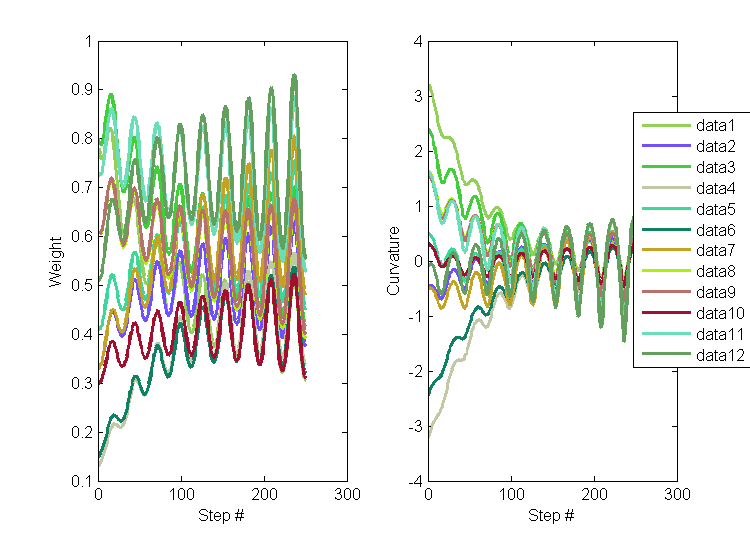
\includegraphics[scale = 0.65]{Pictures3/kHatResult.png}
\caption{An example using our notion of $\hat{K}$. Weights and curvatures were unable to converge, and crashed the program shortly after. Each curve represents a different vertex.}
\label{kHat}
\end{figure}

\end{itemize}

 In the end, we decided to try an equation that took the good aspects of our first trial while broadening its range of stability as we had hoped with the second one. We came up with the equation

\begin{equation}
\label{SRicciN}
\frac{dr_i}{dt} = \overline{K}r_i - K_i\sin(r_i).
\end{equation}

 This equation was derived by applying (\ref{ref1}) to the standard spherical equation and recognizing that the average curvature component should likely not be the sine of the weight, but just the product with the weight itself. Unfortunately, we have no proof that this equation is related to the normalized Euclidean flow. However, in examining its behavior with various triangulations, we found that this one works very well, and acted similarly to that of the normalized Euclidean flow. We find that spheres converge to zero curvature and weights first group together and then approach optimal weights. See Figure~\ref{SphGood}.

 In dealing with vertex transitive triangulations, ones in which each vertex has the same degree, we noted that sometimes all weights would converge to a specific value that was dependent on the number of vertices, and sometimes all the weights would be close to this number but off by a small amount. In either case, the resulting surface area at the end turned out to be $4\pi$. For a vertex transitive genus 0 surface, we found that the preferred weight that each vertex approached was equal to 

$$r_i = \frac{1}{2}\arccos(\frac{\cos(Z)}{1 - \cos(Z)}) \mbox{ where } Z = \frac{\pi(4 + F)}{3F}$$

 and $F$ is the number of faces of the given triangulation. For example, with a tetrahedron, $F = 4, Z = \frac{2\pi}{3},$ and $r_i = \frac{1}{2}\arccos(-\frac{1}{3}) \approx 0.9553.$ 

 We found that this equation does fail if some weights got too large, and the computation time required to reach a stable equilibrium was lengthier than expected. Looking at Fig.~\ref{SphGood}, we see that with a $dt$ size of $0.5$, it took over 500 steps for the system to reach equilibrium, and this would be much longer with the $dt$ used in $\S\ref{InitialResults}$.  

\begin{figure}[ht]
\centering
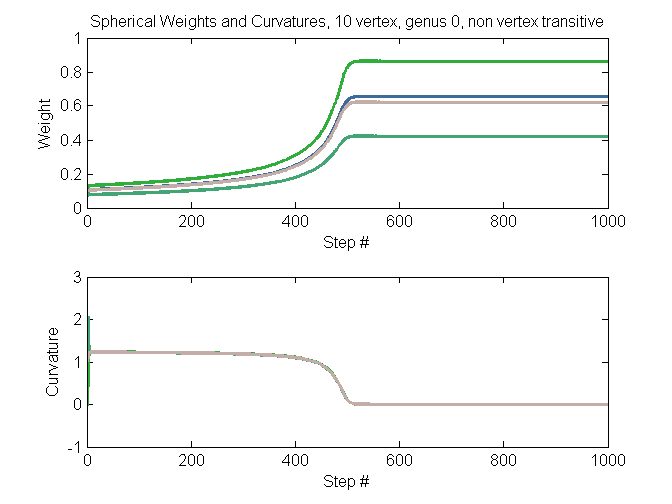
\includegraphics[scale = 0.8]{Pictures3/SphG0V10.png}
\caption{An example of a solution using Eq.~(\ref{SRicciN}). Starting off with equal initial weights of 0.1, vertices merge into one of four groups as they approach uniform curvature relatively quickly. As curvature drops to zero, slowly at first but more quickly as time passes, the weight groups separate from each other to obtain their final weight. In this trial, $dt = 0.50$ to show the complete process.}
\label{SphGood}  
\end{figure}

\subsection{Hyperbolic flow}

In hyperbolic geometry, we encounter a new background that has properties both similar and distinct from Euclidean and spherical systems. A common way to visualize the hyperbolic plane can be seen in Fig.~\ref{PD}. This representation is often called the Poincar\'{e} disk, named after the same Poincar\'{e} as in $\S$\ref{RBk}.

 The hyperbolic plane has several interesting properties. For a line $l$ and a point $P$ not on that line, there are an infinite number of lines through $P$ that do not intersect $l$. In Euclidean geometry, such a line is unique. The shortest distance between two points is still a straight line, but illustratively can be found by following a curved path along a circle centered at infinity going through both points. A more thorough exposition on hyperbolic geometry can be found in most college geometry textbooks.

 In terms of the formulas, they remain relatively similar in format to the spherical equations, except there are two main substitutions. The cosine and sine functions are often replaced with their hyperbolic counterparts $cosh$ and $sinh$, defined as
\begin{eqnarray*}
\sinh(x) &=& \frac{e^x - e^{-x}}{2}\\
\cosh(x) &=& \frac{d\sinh(x)}{dx} = \frac{e^x + e^{-x}}{2}.
\end{eqnarray*}

 The equation for combinatorial Ricci flow is now
\begin{equation}
\label{HRiccif}
\frac{dr_i}{dt} = -K_i\sinh(r_i)
\end{equation}
 

 Like in the case of spherical flow, the average and total curvatures need not remain constant. For a surface, $X$, the average curvature is
$$\overline{K} = \frac{\sum{K_i}}{|V|} = \frac{2\pi\chi + \mbox{Surface Area of }X}{|V|}.$$

\begin{figure}
\centering
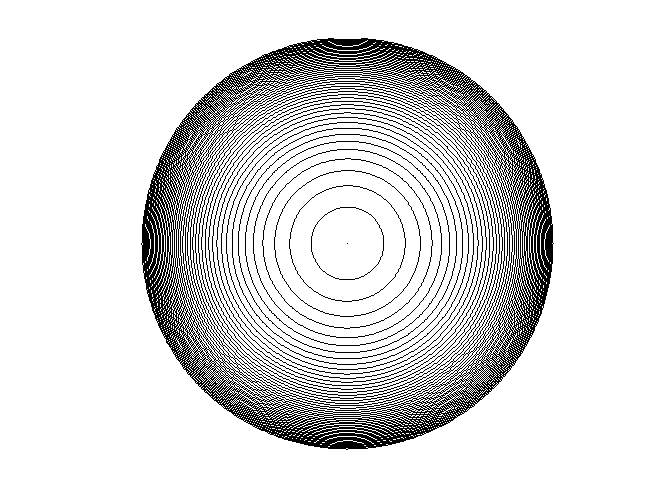
\includegraphics[scale = 0.5]{Pictures3/pDisk.png}
\caption{An illustration of the hyperbolic plane using the Poincar\'{e} disk. All concentric circles are evenly spaced apart in a hyperbolic background, but the outer edge of the disk approaches infinity, so the circles appear closer together.}
\label{PD}
\end{figure}

 After running the hyperbolic Ricci flow on a few samples, we noted that the weights did not always go to zero, as was the case with other unnormalized systems. So in some cases, it almost seems as if this equation is already normalized. Curvatures would converge to zero, and optimum, nonzero weights are achieved in a relatively short time. Other times it behaved like both Euclidean and spherical. Weights would become chaotically large or drop to zero.  

\subsection{Comparison of Systems}

When we began looking into these background geometries, we thought that it would be a good idea to run uniform tests on all three systems. We could observe whether or not each triangulation converges in the same fashion, or if it matters which geometry we choose. If we do discover that all systems behave the same way, we would then like to focus on one geometry, most likely Euclidean. However, since our equation for normalized spherical Ricci flow is not wholly confirmed as the best method, and as the hyperbolic flow may or may not already be normalized, we can not make any strong conclusions on the normalized flows. We did decide, however, to take a look at the behaviors on various manifolds by using the unnormalized equations, (\ref{Riccif}), (\ref{SRiccif}), and (\ref{HRiccif}). We will look at three triangulations, each of a different genus, without performing any morphs, and compare results between each system. 

 In terms of programming these new flows, we were able to adapt our $calcFlow$ program into two new programs, $sphericalCalcFlow$ and $hyperbolicCalcFlow$, to easily distinguish which background we were using. This way we could run the systems one at a time and observe differences in their behaviors in cases with the same initial conditions. 

 \textit{Example:} 12 vertex sphere, vertex transitive of degree 5

 Euclidean- As expected, we obtain a surface where all the vertices attain the same curvature of $\frac{\pi}{3}$ after multiple trials of various weights. The weights appeared to group together as in the normalized spherical case, but they were all decreasing towards zero.

 Spherical- We found that the system was truly stable with nonzero final weights if and only if all initial weights were set exactly to its preferred weight, which is $\approx$ 0.55357 based on the fact that this triangulation has 20 faces. If the initial curvature was below zero, the weights would increase rapidly until the program crashed. If the initial curvature was positive, the vertices would approach the same curvature as in the Euclidean case. In doing so, the weights would drop to zero.

 Hyperbolic- We found that the vertices react in a similar manner to the Euclidean case. They approach the same curvature of $\frac{\pi}{3}$ and drop towards zero weights at the same rate. 

 \textit{Example:} 9 vertex, one-holed torus

 Euclidean- Since we know that $\chi = 0$ for a one-holed torus, we also know that $\overline{K} = 0$ and so each vertex obtains zero curvature. The weights do not drop to zero, but converge to positive values. 

 Spherical- We found this system to be very unstable with the torus. If the initial weights were too large, the total curvature would be well below zero, and the weights would continually increase until sphericalCalcFlow crashed. While we hoped that reducing the initial weights would bring stability to the system, we ended up with the same result.

 Hyperbolic- While the total curvature of the system goes to zero, the weights also approach zero but try to attain the same proportion as the final Euclidean weights. Another thing we noted was the time required for the weights and curvatures to go to zero. This system was extremely slow and took much longer than either the Euclidean or spherical trials. 

 \textit{Example:} 11 vertex, two-holed torus

 Euclidean- As in previous cases, the vertices converge to a uniform curvature. However, as this value was negative (given $\chi = -2$) we saw the weights increase without bound. As there is no limit to the weights in the Euclidean case, $calcFlow$ had no troubles calculating each iteration, but having unbounded weights is still an undesired result. 

 Spherical- Regardless of the initial weights, we found that the total curvature of the system would continually decrease, and as such the weights of each vertex would increase until sphericalCalcFlow crashed. 

 Hyperbolic- Here we found that hyperbolic geometry was very effective. In a very short time, we saw the vertices reach zero curvature, and the weights converge to nonzero values. This is how we got our notion that the hyperbolic Ricci flow was already normalized. This also coincides with the suggestion in \cite{chowluo}; when working with a negative Euler characteristic manifold, one should use hyperbolic geometry.

 To conclude, we conjecture that certain flows work best for triangulations whose total curvature goes to zero in that particular system. 

\begin{itemize}
\item Euclidean is best for systems of genus 1, or one-holed tori. As seen in the second example, the weights of the unnormalized system converged to nonzero values. 
\item Spherical combinatorial Ricci flow works best on manifolds of genus 0, or anything topologically equivalent to a sphere. This is because we have a positive $\chi$ value, so for total curvature to go to 0, the total surface area must go to $4\pi$. Spherical was the only system that produced a nontrivial solution in our first example. 
\item Hyperbolic Ricci flow is best suited for triangulations with a genus of 2 or more. We can see that these systems will be able to reach zero total curvature with a large enough surface area. 
\end{itemize}

\section{Future work}
\label{Future}

\subsection{Linking Delaunay to Ricci flow}
Delaunay surfaces and combinatorial Ricci flows can seem to be very separate concepts, and in many ways with our program structure, they are. Yet there is the possibility of combining both of them to explore other mathematical inquiries. For instance, how does the idea of Delaunay triangles interact with triangulations on a manifold? We know that a circle packed triangulation is weighted Delaunay, but what if the triangulation is not circle packed? Will the Ricci flow lead to a weighted Delaunay triangulation?

\subsection{Circle packing expansions}
\label{circExt}

Circle packing is but a very special way to characterize our side lengths. If we relax this criteria and let the circles overlap, we can introduce a second weight $\Phi$ that is representative of the angle of their intersection. See Figure \ref{fig:intcirc}. If we let $\Phi$ be constant, we can then evaluate our side lengths as $$l_{ij} = \sqrt{r_i^2 + r_j^2 + 2r_ir_j\cos(\Phi(e_{ij}))}$$ With this more general interpretation, we can examine questions asked by Chow and Luo in \cite{chowluo}.

\begin{figure}
\begin{center}
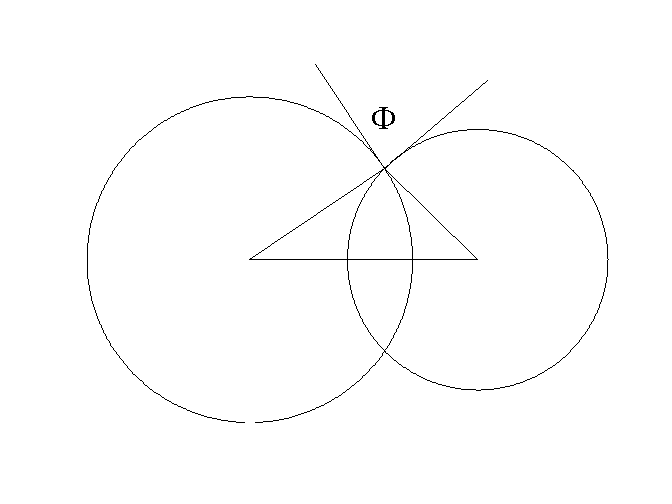
\includegraphics[scale = 0.6]{Pictures3/intcirc2.png}
\end{center}
\caption{An example of relaxing circle packing and introducing $\Phi.$}
\label{fig:intcirc}
\end{figure}

\subsection{Spherical and hyperbolic extensions}
While we investigated various tests to compare the three combinatorial Ricci flows, we would like to investigate spherical and hyperbolic even further. Primarily, we would like to determine if our normalized equation, Eq.~(\ref{SRicciN}) is related to the Euclidean normalized flow or determine if a true normalized flow exists. Likewise, we would like to investigate the existence of a normalized hyperbolic flow that behaves like the Euclidean version. We would also like to implement a scaling notion per vertex in the spherical case so that the weights could increase without necessarily crashing the program. 

\subsection{3-Dimensional triangulations}
Triangulations exist outside of two dimensions and one future goal is to perform flows in a three dimensional setting. The flow in this case is known as Yamabe flow, discussed in \cite{DrG}. While Yamabe flow is similar to Ricci flow, its value of $K_i$ is determined quite differently, involving not only the angles of the faces, but also the cone angles associated with tetrahedron vertices. The structure is in place from this project to accomplish this goal. To help the understanding of both the two and three dimensional triangulations, we would like to create a way to visualize them and explore the surfaces locally.

\section{Conclusion}

There were many things we wanted to explore with triangulations, particularly towards Delaunay surfaces and combinatorial Ricci flow. A major aspect of our research was the creation of a functional and adaptable program to provide meaningful data. We feel that we have accomplished this goal. We have added a user interface to the program (see $\S\ref{calcFlowCode}$) for a straightforward way to run flips or flows. We hope that in the future this program can be used by others to perform their own tests.

 Our work on Delaunay surfaces is unfinished, but we are excited about the prospects introduced by negative triangles. The research performed in this paper is the beginning of what we hope is a development of these negative triangles and of universally accepted definitions about them. In combinatorial Ricci flow, we have helped confirm the assertions given by \cite{chowluo} with numerical results in the Euclidean case. We have seen how certain properties of a weighted triangulation behave under combinatorial Ricci flow such as the weights and curvatures. Under Spherical geometry we remain uncertain as to the validity of our normalized Ricci flow, but are optimistic that such a formula does exist. Along with the above mentioned areas of further work, we also propose research in 3-dimensional Yamabe flow and in Delaunay algorithms on manifolds.

 In addition to the clearly defined goals in the paper, we were able to experience a large scale project that often required independent work. We also became knowledgeable in an area of mathematics that is still young in its development. For these things we would like to thank Dr. David Glickenstein for being our mentor and guide on this project, Dr. Robert Indik and the University of Arizona Math Department for their help and support, and National Science Foundation VIGRE $\#$0602173.

\newpage
\bibliography{Test1}  
\bibliographystyle{plain}

\newpage
\appendix
\section{Appendix}

\subsection{Derivation of Eq.~(\ref{proof1})}
\maketitle
	
	We used the criterion $$f(\tilde{r_1},\tilde{r_2},\ldots,\tilde{r_n}) = \prod{\tilde{r_i}} = \prod{\alpha r_i} = \alpha^n\prod{r_i}= C$$ to constrain the values of radii. We take the derivative of $f$ with respect to $t$ and obtain
	\begin{eqnarray*}
	\frac{df}{dt} & = & n\alpha^{n-1}\frac{d\alpha}{dt}r_1r_2\ldots r_n + \alpha^n\frac{dr_1}{dt}r_2r_3\ldots r_n\\
								& + & \alpha^nr_1\frac{dr_2}{dt}r_3r_4\ldots r_n + \ldots + \alpha^nr_1r_2\ldots r_{n-1}\frac{dr_n}{dt}.
	\end{eqnarray*}
	But since $\displaystyle \frac{dr_i}{dt} = -K_ir_i$ from Eq.~(\ref{Riccif}) we obtain
	\begin{eqnarray*}
	\frac{df}{dt} & = & \frac{n\alpha^{n}}{\alpha}\frac{d\alpha}{dt}r_1r_2\ldots r_n - K_1\alpha^nr_1r_2r_3\ldots r_n\\
								& - & K_2\alpha^nr_1r_2r_3r_4\ldots r_n - \ldots - K_n\alpha^nr_1r_2\ldots r_{n-1}r_n
	\end{eqnarray*}
	from which we can group terms and obtain
	\begin{eqnarray*}
	\frac{df}{dt} & = & (\alpha^nr_1r_2\ldots r_n)(\frac{n}{\alpha}\frac{d\alpha}{dt} - K_1 - K_2 - \ldots - K_n)\\
								& = & C(\frac{n}{\alpha}\frac{d\alpha}{dt} - K_1 - K_2 - \ldots - K_n).
	\end{eqnarray*}
	If we assume the product is a constant, we have $\displaystyle \frac{df}{dt} = 0.$ Thus we have $$\frac{n}{\alpha}\frac{d\alpha}{dt} - K_1 - K_2 - \ldots - K_n = 0.$$
	Rearranging we have
$$\frac{1}{\alpha}\frac{d\alpha}{dt} = \frac{d(\log \alpha)}{dt} = \frac{K_1 + K_2 + \ldots + K_n}{n} = \overline{K}$$
	which we refer to as Eq.~(\ref{proof1})

\begin{figure}
\label{NonDelPropfig}
\centering
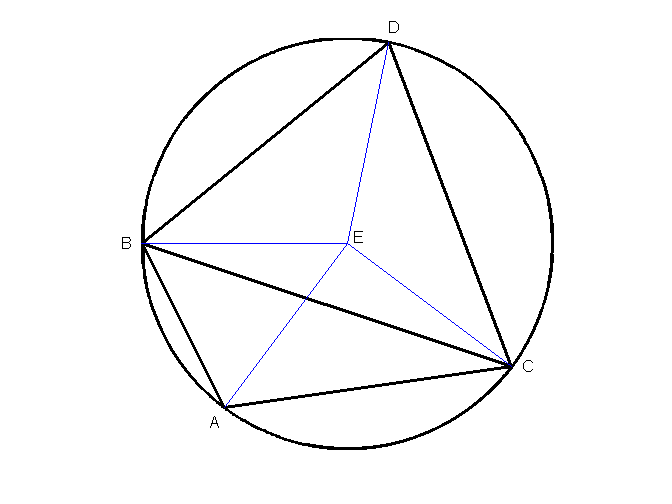
\includegraphics[scale = 0.5]{Pictures3/geometryU.png}
\caption{An illustration associated with our proof of Proposition \ref{NonDelProp}.}
\end{figure}

\subsection{Proof of Proposition \ref{NonDelProp}}
The sum of the opposite angles on a non-Delaunay hinge is greater than $\pi$.
\begin{proof}
\label{prop1}
Let $\Delta ABC$ and $\Delta BCD$ be triangles with common edge $\overline{BC}$ (see fig. \ref{NonDelPropfig}). Let $r$ be the radius of the circumcircle of  $\Delta ABC$ and $E$ be the center of that circle. Then we wish to show that if $\overline{DE}$ is less than $r$, then $\angle BAC + \angle BDC > \pi$.

We know that $\overline{BE}=\overline{AE}=\overline{EC}=r$, so $\angle EBA = \angle BAE$ and $\angle EAC = \angle ACE$. Therefore, $\angle EBA + \angle ACE= \angle BAC$.

We first consider $\overline{DE}=r$. Then similar to above, $\angle EBD = \angle BDE$ and $\angle EDC = \angle DCE$, so $\angle EBD + \angle DCE= \angle BDC$. Thus, $\angle BAC + \angle EBA + \angle ACE + \angle BDC + \angle EBD + \angle DCE = 2\angle BAC + 2\angle BDC = 2\pi$
since $ABCD$ is a quadrilateral. So $\angle BAC + \angle BDC = \pi$.

Now we suppose $\overline{DE}$ is less than $r$. So $\angle BDE > \angle EBD$ and $\angle DCE > \angle EDC$. Therefore we have
\begin{align*}
\angle BAC + \angle EBA + \angle ACE + \angle BDC + \angle EBD + \angle DCE = 2\pi \\
\Rightarrow 2\angle BAC + 2\angle BDC > 2\pi \quad \Rightarrow \angle BAC + \angle BDC > \pi.
\end{align*}

 Hence the sum of the opposite angles on a non-Delaunay hinge is greater than $\pi$. \qedhere
\end{proof}

\begin{figure}
\label{weidelpropfig}
\centering
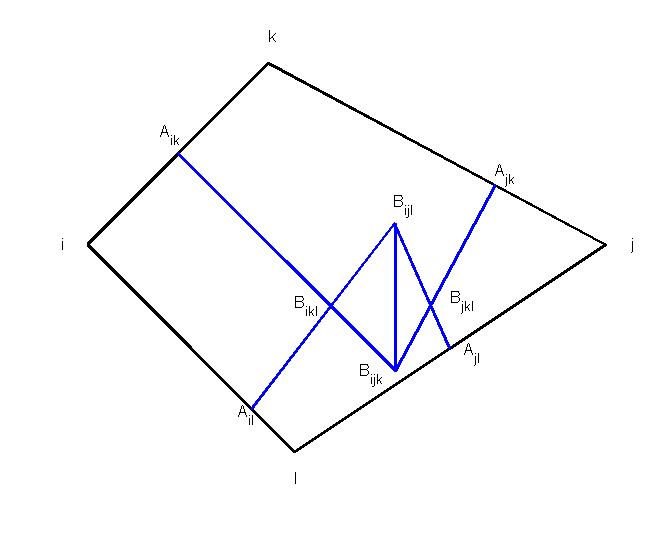
\includegraphics[scale = 0.45]{Pictures3/geometryW3.png}
\caption{An illustration associated with our proof of Proposition \ref{NonDelProp}.}
\end{figure}

\subsection{Proof of Proposition \ref{weidelprop}}
Any hinge that is non-weighted-Delaunay will become weighted Delaunay after a 2-2 flip is performed on it.
\begin{proof}
\label{prop2}

Consider the hinge consisting of edge $\{i, j\}$ and faces $\{i, j, k\}$ and $\{i, j, l\}$. Assume this hinge is non-weighted-Delaunay. Let $A_{ik} = C(\{i, k\})$, $A_{il} = C(\{i, l\})$, $A_{jk} = C(\{j, k\})$, and $A_{jl} = C(\{j, l\})$.
Let $B_{ijk} = C(\{i, j, k\})$ and $B_{ijl} = C(\{i, j, l\})$. If we draw the dual, $\overline{B_{ijk}B_{ijl}}$, we know that the length of the dual is negative and perpendicular to $\{i, j\}$. We can also say that $B_{ijk}$ lies on the side of $l$ and $B_{ijl}$ lies on the side of $k$. 

Now conider the hinge when the edge has been flipped. We now have edge $\{k, l\}$ and faces $\{i, l, k\}$ and $\{j, l, k\}$.
Let $B_{ikl} = C(\{i, k, l\})$ and $B_{jkl} = C(\{j, k, l\})$. Draw $\overline{A_{ik}B_{ijk}}$, $\overline{A_{jk}B_{ijk}}$, $\overline{A_{il}B_{ijl}}$, and $\overline{A_{jl}B_{ijl}}$. We know that $\overline{A_{ik}B_{ijk}}$ and $\overline{A_{il}B_{ijl}}$ intersect at $B_{ikl}$ and $\overline{A_{jk}B_{ijk}}$ and $\overline{A_{jl}B_{ijl}}$ intersect at $B_{jkl}$. We can draw the dual of $\{k, l\}$, $\overline{B_{ikl}B_{jkl}}$, and we know that $B_{ikl}$ lies on the side of $i$ and $B_{jkl}$ lies on the side of $j$. This means that the dual must have positive length.\qedhere

\end{proof}

\subsection{Remarks on Runge-Kutta method for solving Eq.~(\ref{Riccin})}

The method used by Moreau in \cite{JPM} to solve a differential equation involves using a Runge-Kutta method. Prior to adapting the code from Moreau's website, we reached the conclusion that a Runge-Kutta format would be most beneficial for this type of differential equation problem. Even though it is more computationally complex than the simpler Euler's method, it makes up in its ability to converge and in its accuracy. According to $\cite{DiffEq}$ the error associated with using Runge-Kutta is on the order of $h^4$, whereas with a standard Euler approximation the error is simply of order $h$, with $h = dt$ being our step incremental.

Based on our evaluations of radii and curvatures over time, it appears to converge exponentially for each vertex. However, as mentioned previously, performing flips on a triangulation may create unusual behavior.

\subsection{Data Plots}
\label{dataplots}

\begin{figure}[ht]
\centering
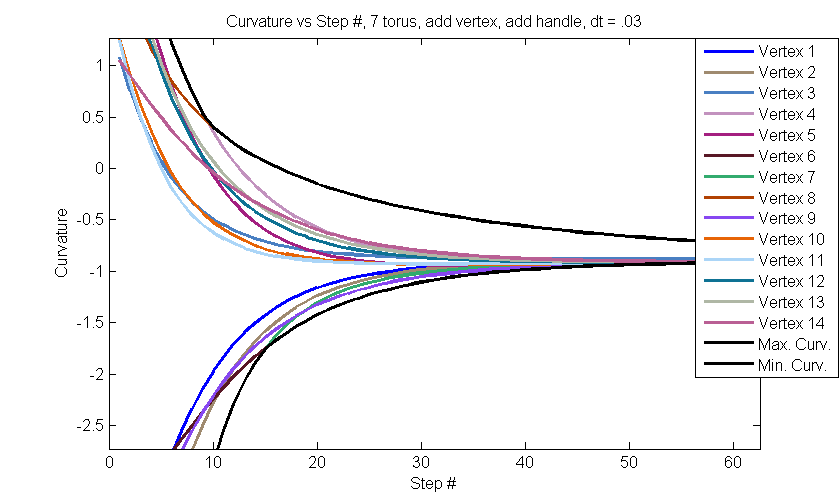
\includegraphics[scale = 0.8]{Pictures3/curvcurves.png}
\caption{An example of curvatures over time. While they do converge to the same curvature, the vertex with the maximum or minimum curvature may change. This is a separate trial than that producing Fig.~\ref{fig:t7vh}}
\end{figure}

\begin{figure}[ht]
\begin{center}
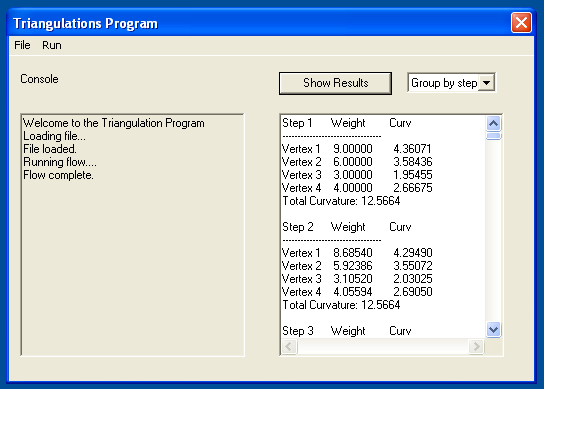
\includegraphics[scale = 0.65]{Pictures3/GUIpic.png}
\caption{A snapshot of the user interface written to run both Ricci flows and Delaunay flip algorithms. Results of a flow are written in a text field on the right.}
\end{center}
\end{figure}

%\newpage
\subsection{Code Examples}
Code from the program can be found here: http://code.google.com/p/geocam. 
 
The \textit{calcFlow} method calculates the combinatorial Ricci flow of the current Triangulation using the Runge-Kutta method. Results from the steps are written into vectors of doubles provided. The parameters are:

\begin{itemize}
\item\textbf{vector$<$double$>$* weights-} A vector of doubles to append the results of weights, grouped by step, with a total size of numSteps * numVertices.
\item\textbf{vector$<$double$>$* curvatures-} A vector of doubles to append the results of curvatures, grouped by step, with a total size of numSteps * numVertices. The time step size. Initial and ending times not needed since diff. equations are independent of time.
\item\textbf{double* initWeights-} Array of initial weights of the Vertices in order.
\item\textbf{int numSteps-} The number of steps to take. (dt = (tf - ti)/numSteps)
\item\textbf{bool adjF-} Boolean of whether or not to use adjusted differential equation. True to use adjusted.
\end{itemize}

 The information placed in the vectors are the weights and curvatures for each Vertex at each step point. The data is grouped by steps, so the first vertex of the first step is the beginning element. After n doubles are placed, for an n-vertex triangulation, the first vertex of the next step follows. If the vectors passed in are not empty, the data is added to the end of the vector and the original information is not cleared.

\label{calcFlowCode}
\begin{verbatim}
void calcFlow(vector<double>* weights, vector<double>* curvatures, double dt, 
              double* initWeights, int numSteps, bool adjF)  
{
  int p = Triangulation::vertexTable.size(); // The number of vertices or 
                                             // number of variables in system.
                                         
  double ta[p],tb[p],tc[p],td[p],z[p]; // Temporary arrays to hold data for 
                                      // the intermediate steps in.
  int    i,k; // ints used for "for loops". i is the step number,
              // k is the kth vertex for the arrays.
  map<int, Vertex>::iterator vit; // Iterator to traverse through the vertices.
  // Beginning and Ending pointers. (Used for "for" loops)
  map<int, Vertex>::iterator vBegin = Triangulation::vertexTable.begin();
  map<int, Vertex>::iterator vEnd = Triangulation::vertexTable.end();
  
  double net = 0; // Net and prev hold the current and previous
  double prev;    //  net curvatures, respectively.
   for (k=0; k<p; k++) {
    z[k]=initWeights[k]; // z[k] holds the current weights.
   }
   for (i=1; i<numSteps+1; i++)
   {  // This is the main loop through each step.
    prev = net; // Set prev to net.
    net = 0;    // Reset net.
    
       for (k=0, vit = vBegin; k<p && vit != vEnd; k++, vit++)  
       {
           // Set the weights of the Triangulation.
           vit->second.setWeight(z[k]);
       }
       if(i == 1) // If first time through, use static method to 
       {           // calculate total curvature.
            prev = Triangulation::netCurvature();
       }
       for (k=0, vit = vBegin; k<p && vit != vEnd; k++, vit++) 
       {  // First "for loop"in whole step calculates everything manually.
           (*weights).push_back( z[k]); // Adds the data to the vector.
           double curv = curvature(vit->second);
           if(curv < 0.00005 && curv > -0.00005) 
           {  // Adjusted for small numbers. We want it to print nicely.
             (*curvatures).push_back(0.); // Adds the data to the vector.
           }
           else {
               (*curvatures).push_back(curv);
           }
           net += curv; // Calculating the net curvature.
           // Calculates the differential equation, either normalized or
           // standard.
           if(adjF) ta[k]= dt * ((-1) * curv 
                           * vit->second.getWeight() +
                           prev /  p
                           * vit->second.getWeight());
           else     ta[k] = dt * (-1) * curv 
                           * vit->second.getWeight();
           
       }
       for (k=0, vit = vBegin; k<p && vit != vEnd; k++, vit++)  
       { // Set the new weights to our triangulation.
           vit->second.setWeight(z[k]+ta[k]/2);
       }
       for (k=0, vit = vBegin; k<p && vit != vEnd; k++, vit++)  
       {
            // Again calculates the differential equation, but we
            // still need the data in ta[] so we use tb[] now.
            if(adjF) tb[k]=dt*adjDiffEQ(vit->first, net);
            else     tb[k]=dt*stdDiffEQ(vit->first);
       }
       for (k=0, vit = vBegin; k<p && vit != vEnd; k++, vit++)  
       { // Set the new weights.
           vit->second.setWeight(z[k]+tb[k]/2);
       }
       for (k=0, vit = vBegin; k<p && vit != vEnd; k++, vit++)  
       {
            if(adjF) tc[k]=dt*adjDiffEQ(vit->first, net);
            else     tc[k]=dt*stdDiffEQ(vit->first);
       }
       for (k=0, vit = vBegin; k<p && vit != vEnd; k++, vit++)  
       { // Set the new weights.
           vit->second.setWeight(z[k]+tc[k]);
       }
       for (k=0, vit = vBegin; k<p && vit != vEnd; k++, vit++)  
       {
            if(adjF) td[k]=dt*adjDiffEQ(vit->first, net);
            else     td[k]=dt*stdDiffEQ(vit->first);
       }
       for (k=0; k<p; k++) // Adjust z[k] according to algorithm.
       {
         z[k]=z[k]+(ta[k]+2*tb[k]+2*tc[k]+td[k])/6;
         
       }
   }
}
\end{verbatim}

\section*{About the authors}

Alex Henniges is a junior double majoring in Math and Computer Science. Thomas Williams is a senior in Comprehensive Mathematics with a minor in Computer Science and a background in Math Education. Mitch Wilson is a senior double majoring in Applied Math and Mechanical Engineering.

 Contact information:
\begin{itemize}
\item Dr. David Glickenstein- glickenstein@math.arizona.edu
\item Alex Henniges- henniges@email.arizona.edu
\item Thomas Williams- thwillia@email.arizona.edu
\item Mitch Wilson- mjw@email.arizona.edu
\end{itemize}

\end{document}